% This is a modified version of the tufte-latex book example in which the title page and the contents page resemble Tufte's VDQI book, using Kevin Godby's code from this thread at https://groups.google.com/forum/#!topic/tufte-latex/ujdzrktC1BQ.
%% Unfortunately for the contents to contain
%% the "Parts" lines successfully, hyperref
%% needs to be disabled.
\documentclass[nohyper,nobib,a4paper]{tufte-book}
\usepackage{nameref}
\usepackage{minted} %Code
\usepackage{algorithm} %Note: remove if errors
%\usepackage{algorithmic} %Note: remove if errors
\usepackage{algpseudocode}
\usepackage[dutch]{babel}
% \hypersetup{colorlinks}% uncomment this line if you prefer colored hyperlinks (e.g., for onscreen viewing)
%
\usepackage{ dsfont } % for fancy Z and R and N 
\usepackage{amsmath}
\DeclareMathOperator\supp{supp}
\DeclareMathOperator\conf{conf}
\DeclareMathOperator\MIS{MIS}
%
% \usepackage{hyphenat}
\usepackage{url}
\usepackage[backend=biber, natbib=true, style=numeric]{biblatex}
\addbibresource{bib.bib}
\usepackage{xargs}
\renewcommandx{\cite}[3][1={0pt},2={}]{\sidenote[][#1]{\fullcite[#2]{#3}}}

%%
% Book metadata
\title{Internetapplicaties}
\date{}
\author[Pieter Delobelle Anton Danneels]{Pieter Delobelle \\ Anton Danneels}
\publisher{KU Leuven}

%%
% If they're installed, use Bergamo and Chantilly from www.fontsite.com.
% They're clones of Bembo and Gill Sans, respectively.
%\IfFileExists{bergamo.sty}{\usepackage[osf]{bergamo}}{}% Bembo
%\IfFileExists{chantill.sty}{\usepackage{chantill}}{}% Gill Sans

%\usepackage{microtype}

%%
% Just some sample text
\usepackage{lipsum}

%%
% For nicely typeset tabular material
\usepackage{booktabs}

%%
% For graphics / images
\usepackage{graphicx}
\setkeys{Gin}{width=\linewidth,totalheight=\textheight,keepaspectratio}
\graphicspath{{graphics/}}

% The fancyvrb package lets us customize the formatting of verbatim
% environments.  We use a slightly smaller font.
\usepackage{fancyvrb}
\fvset{fontsize=\normalsize}

%%
% Prints argument within hanging parentheses (i.e., parentheses that take
% up no horizontal space).  Useful in tabular environments.
\newcommand{\hangp}[1]{\makebox[0pt][r]{(}#1\makebox[0pt][l]{)}}

%%
% Prints an asterisk that takes up no horizontal space.
% Useful in tabular environments.
\newcommand{\hangstar}{\makebox[0pt][l]{*}}

%%
% Prints a trailing space in a smart way.
\usepackage{xspace}

%\usepackage{amsmath}

%%
% Some shortcuts for Tufte's book titles.  The lowercase commands will
% produce the initials of the book title in italics.  The all-caps commands
% will print out the full title of the book in italics.
\newcommand{\vdqi}{\textit{VDQI}\xspace}
\newcommand{\ei}{\textit{EI}\xspace}
\newcommand{\ve}{\textit{VE}\xspace}
\newcommand{\be}{\textit{BE}\xspace}
\newcommand{\VDQI}{\textit{The Visual Display of Quantitative Information}\xspace}
\newcommand{\EI}{\textit{Envisioning Information}\xspace}
\newcommand{\VE}{\textit{Visual Explanations}\xspace}
\newcommand{\BE}{\textit{Beautiful Evidence}\xspace}

\newcommand{\TL}{Tufte-\LaTeX\xspace}

% Prints the month name (e.g., January) and the year (e.g., 2008)
\newcommand{\monthyear}{%
  \ifcase\month\or January\or February\or March\or April\or May\or June\or
  July\or August\or September\or October\or November\or
  December\fi\space\number\year
}


% Prints an epigraph and speaker in sans serif, all-caps type.
\newcommand{\openepigraph}[2]{%
  %\sffamily\fontsize{14}{16}\selectfont
  \begin{fullwidth}
  \sffamily\large
  \begin{doublespace}
  \noindent\allcaps{#1}\\% epigraph
  \noindent\allcaps{#2}% author
  \end{doublespace}
  \end{fullwidth}
}

% Inserts a blank page
\newcommand{\blankpage}{\newpage\hbox{}\thispagestyle{empty}\newpage}

\usepackage{units}

% Typesets the font size, leading, and measure in the form of 10/12x26 pc.
\newcommand{\measure}[3]{#1/#2$\times$\unit[#3]{pc}}

% Macros for typesetting the documentation
\newcommand{\hlred}[1]{\textcolor{Maroon}{#1}}% prints in red
\newcommand{\hangleft}[1]{\makebox[0pt][r]{#1}}
\newcommand{\hairsp}{\hspace{1pt}}% hair space
\newcommand{\hquad}{\hskip0.5em\relax}% half quad space
\newcommand{\TODO}{\textcolor{red}{\bf TODO!}\xspace}
\newcommand{\ie}{\textit{i.\hairsp{}e.}\xspace}
\newcommand{\eg}{\textit{e.\hairsp{}g.}\xspace}
\newcommand{\na}{\quad--}% used in tables for N/A cells
\providecommand{\XeLaTeX}{X\lower.5ex\hbox{\kern-0.15em\reflectbox{E}}\kern-0.1em\LaTeX}
\newcommand{\tXeLaTeX}{\XeLaTeX\index{XeLaTeX@\protect\XeLaTeX}}
% \index{\texttt{\textbackslash xyz}@\hangleft{\texttt{\textbackslash}}\texttt{xyz}}
\newcommand{\tuftebs}{\symbol{'134}}% a backslash in tt type in OT1/T1
\newcommand{\doccmdnoindex}[2][]{\texttt{\tuftebs#2}}% command name -- adds backslash automatically (and doesn't add cmd to the index)
\newcommand{\doccmddef}[2][]{%
  \hlred{\texttt{\tuftebs#2}}\label{cmd:#2}%
  \ifthenelse{\isempty{#1}}%
    {% add the command to the index
      \index{#2 command@\protect\hangleft{\texttt{\tuftebs}}\texttt{#2}}% command name
    }%
    {% add the command and package to the index
      \index{#2 command@\protect\hangleft{\texttt{\tuftebs}}\texttt{#2} (\texttt{#1} package)}% command name
      \index{#1 package@\texttt{#1} package}\index{packages!#1@\texttt{#1}}% package name
    }%
}% command name -- adds backslash automatically
\newcommand{\doccmd}[2][]{%
  \texttt{\tuftebs#2}%
  \ifthenelse{\isempty{#1}}%
    {% add the command to the index
      \index{#2 command@\protect\hangleft{\texttt{\tuftebs}}\texttt{#2}}% command name
    }%
    {% add the command and package to the index
      \index{#2 command@\protect\hangleft{\texttt{\tuftebs}}\texttt{#2} (\texttt{#1} package)}% command name
      \index{#1 package@\texttt{#1} package}\index{packages!#1@\texttt{#1}}% package name
    }%
}% command name -- adds backslash automatically
\newcommand{\docopt}[1]{\ensuremath{\langle}\textrm{\textit{#1}}\ensuremath{\rangle}}% optional command argument
\newcommand{\docarg}[1]{\textrm{\textit{#1}}}% (required) command argument
\newenvironment{docspec}{\begin{quotation}\ttfamily\parskip0pt\parindent0pt\ignorespaces}{\end{quotation}}% command specification environment
\newcommand{\docenv}[1]{\texttt{#1}\index{#1 environment@\texttt{#1} environment}\index{environments!#1@\texttt{#1}}}% environment name
\newcommand{\docenvdef}[1]{\hlred{\texttt{#1}}\label{env:#1}\index{#1 environment@\texttt{#1} environment}\index{environments!#1@\texttt{#1}}}% environment name
\newcommand{\docpkg}[1]{\texttt{#1}\index{#1 package@\texttt{#1} package}\index{packages!#1@\texttt{#1}}}% package name
\newcommand{\doccls}[1]{\texttt{#1}}% document class name
\newcommand{\docclsopt}[1]{\texttt{#1}\index{#1 class option@\texttt{#1} class option}\index{class options!#1@\texttt{#1}}}% document class option name
\newcommand{\docclsoptdef}[1]{\hlred{\texttt{#1}}\label{clsopt:#1}\index{#1 class option@\texttt{#1} class option}\index{class options!#1@\texttt{#1}}}% document class option name defined
\newcommand{\docmsg}[2]{\bigskip\begin{fullwidth}\noindent\ttfamily#1\end{fullwidth}\medskip\par\noindent#2}
\newcommand{\docfilehook}[2]{\texttt{#1}\index{file hooks!#2}\index{#1@\texttt{#1}}}
\newcommand{\doccounter}[1]{\texttt{#1}\index{#1 counter@\texttt{#1} counter}}

% Generates the index
\usepackage{makeidx}
\makeindex

%%%% Kevin Godny's code for title page and contents from https://groups.google.com/forum/#!topic/tufte-latex/ujdzrktC1BQ
\makeatletter
\addto\captionsdutch{\renewcommand{\ALG@name}{Algoritme}}
\renewcommand{\maketitlepage}{%
\begingroup%
\setlength{\parindent}{0pt}

{\fontsize{24}{24}\selectfont\textit{\@author}\par}

\vspace{1.75in}{\fontsize{36}{54}\selectfont\@title\par}

\vspace{0.5in}{\fontsize{14}{14}\selectfont\textsf{\smallcaps{\@date}}\par}

\vfill{\fontsize{14}{14}\selectfont\textit{\@publisher}\par}

\thispagestyle{empty}
\endgroup
}
\makeatother

\titlecontents{part}%
    [0pt]% distance from left margin
    {\addvspace{0.25\baselineskip}}% above (global formatting of entry)
    {\allcaps{Part~\thecontentslabel}\allcaps}% before w/ label (label = ``Part I'')
    {\allcaps{Part~\thecontentslabel}\allcaps}% before w/o label
    {}% filler and page (leaders and page num)
    [\vspace*{0.5\baselineskip}]% after

\titlecontents{chapter}%
    [4em]% distance from left margin
    {}% above (global formatting of entry)
    {\contentslabel{2em}\textit}% before w/ label (label = ``Chapter 1'')
    {\hspace{0em}\textit}% before w/o label
    {\qquad\thecontentspage}% filler and page (leaders and page num)
    [\vspace*{0.5\baselineskip}]% after

\titlecontents{section}%
    [8em]% distance from left margin
    {}% above (global formatting of entry)
    {\contentslabel{2em}\textit}% before w/ label (label = ``section 1'')
    {\hspace{0em}\textit}% before w/o label
    {\qquad\thecontentspage}% filler and page (leaders and page num)
    [\vspace*{0.3\baselineskip}]% after
%%%% End additional code by Kevin Godby and Pieter Delobelle

\begin{document}

% Front matter
\frontmatter

% r.1 blank page
% \blankpage

% v.2 epigraphs
% \openepigraph{%
% A designer knows that he has achieved perfection 
% not when there is nothing left to add, 
% but when there is nothing left to take away.
% }{Antoine de Saint-Exup\'{e}ry}
% \vfill
% \openepigraph{%
% \ldots the designer of a new system must not only be the implementor and the first 
% large-scale user; the designer should also write the first user manual\ldots 
% If I had not participated fully in all these activities, 
% literally hundreds of improvements would never have been made, 
% because I would never have thought of them or perceived 
% why they were important.
% }{Donald E. Knuth}


% r.3 full title page
\maketitle


% v.4 copyright page
\newpage \thispagestyle{empty}
 \openepigraph{%
I have cleared the Augean stables of astronomy of cycles and spirals, and left behind me a single cartload of dung.
}{---Johannes Kepler%, {\itshape Design, Form, and Chaos}
}
 \vfill
\begin{fullwidth}
~\vfill
\thispagestyle{empty}
\setlength{\parindent}{0pt}
\setlength{\parskip}{\baselineskip}

\includegraphics[width=0.25\textwidth]{res/by-sa.eps}

\smallcaps{\the\year\ Pieter Delobelle en Anton Danneels}

\smallcaps{De inhoud van dit werk valt onder een Creative Commons Naamsvermelding-GelijkDelen 4.0 Internationaal-licentie}  (\url{https://creativecommons.org/licenses/by-sa/4.0}).


\par\smallcaps{Design by tufte-latex.googlecode.com, modifications by Pieter Delobelle}

\par The design is licensed under the Apache License, Version 2.0 (the ``License''); you may not
use this file except in compliance with the License. You may obtain a copy
of the License at \url{http://www.apache.org/licenses/LICENSE-2.0}. Unless
required by applicable law or agreed to in writing, software distributed
under the License is distributed on an \smallcaps{``AS IS'' BASIS, WITHOUT
WARRANTIES OR CONDITIONS OF ANY KIND}, either express or implied. See the
License for the specific language governing permissions and limitations
under the License.\index{license}

\end{fullwidth}

% r.5 contents
\setcounter{tocdepth}{1}
\tableofcontents

%\listoffigures

%\listoftables

% r.9 introduction
\cleardoublepage
\chapter*{Introductie}
Deze cursus hoort bij het vak \emph{internetapplicaties} van Tony Wouters, gegeven op de Technologiecampus Gent van de Katholieke Universiteit van Leuven. 

De broncode van de gebruikte scripts is ook beschikbaar op \url{https://github.com/iPieter/internetapplicaties}.

%%
% Start the main matter (normal chapters)
\mainmatter

% Chapter 1: Web data minig
\chapter{Web data mining}
\section{Waarom data mining}
Met de opkomst van het internet, of meer bepaald het \emph{World Wide Web}, is er een explosie aan nieuwe data beschikbaar gekomen. Het web is een onderdeel geworden van het dagelijkse leven waarbij miljarden mensen met elkaar verbonden zijn via biljoenen documenten. Deze documenten zijn aan elkaar gelinkt via hyperlinks. Hierdoor is een nieuw soort maatschappij ontstaan: de virtuele maatschappij. 

Ondanks deze grote hoeveelheid nieuwe info is er een fenomeen ontstaan waarbij er een grote hoeveelheid data beschikbaar is die eigenlijk niet gebruikt wordt: de \emph{data gap}. De opslag van gegevens wordt steeds goedkoper, maar het analyseren van de data blijkt niet eenvoudig.

Er zijn drie grote elementen die de analyse moeilijk maken. Een eerste component is dat de data, beschikbaar op het internet, vaak geen vaste structuur heeft. Men moet dus eerst de data herwerken zodat men een vast patroon heeft dat gebruikt wordt in een bepaald algoritme.
Een tweede probleem is dat de data vaak veel ruis bevat, data die men niet nodig heeft. 
Tot slot is de data steeds veranderend: het is dynamisch.

Om deze grote hoeveelheid data toch te verwerken gebruikt men \emph{web data mining}. Dit is een automatische manier om informatie en kennis te extraheren uit het web. Deze techniek heeft 3 toepassingen: 
\begin{itemize}
  \item \textbf{Web content mining}: Het analyseren van data op basis van de inhoud van webpagina's.
  \item \textbf{Web usage mining}: Het analyseren van gedragspatronen op basis van de gebruikers logbestanden.
  \item \textbf{Web structure mining}: Het analyseren van het data op basis van hyperlinks.
\end{itemize}
\section{Data mining}
Voor we verder ingaan op het concept van web mining, bekijken we eerst \emph{data mining}. Data mining is het proces om patronen of kennis te ontdekken in databronnen. Het staat daarom ook bekend als KDD: \emph{Knowledge discovery in databases}. Dit proces is multidisciplinair en beslaat domeinen zoals \emph{machine learning}, statistiek, databanken, visualisatie \dots  Het proces is samengevat in de volgende figuur:

\begin{figure}
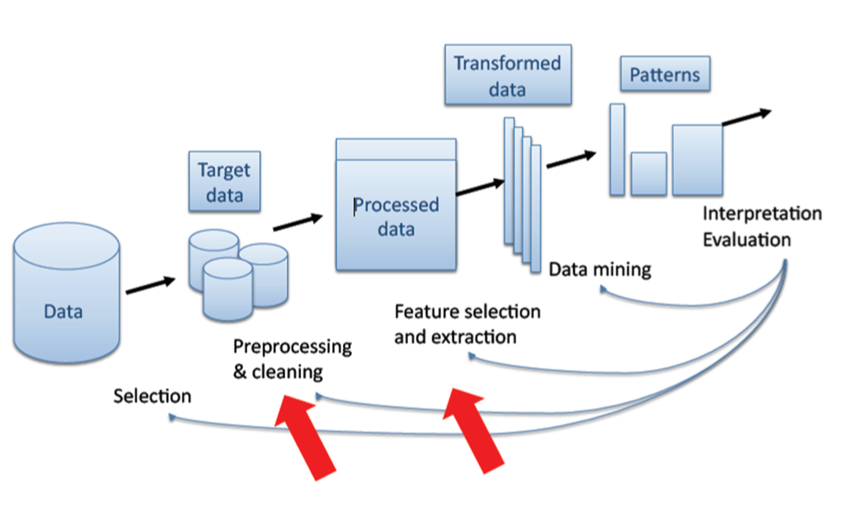
\includegraphics[]{res/kdd_process.png}
\caption{Het data mining proces.}
\end{figure}
Zoals we zien bestaat dit proces uit meerdere stappen.

\begin{enumerate}
\item Eerst wordt de data verzameld. Dit kan uit een database komen of kan bestaan uit verzameling van allemaal bronnen
\item In de tweede stap wordt een selectie gemaakt uit de data. Stel bijvoorbeeld dat we tweets analyseren. Indien we dit opvragen, dan krijgen we extra metadata zoals de locatie en of de tweet een antwoord is op iemand anders. We kunnen er dan voor kiezen om enkel tweets te selecteren die geen antwoord zijn.
\item Vervolgens is er de \emph{data cleaning}-stap. Hierbij wordt ontbrekende info aangevuld of wordt er data weggelaten indien blijkt dat deze niet bruikbaar is.
\item Nadat er enkel schone data overblijft moet deze nog worden omgezet naar data die gebruikt kan worden voor mining. Hierbij gebruikt men technieken zoals aggregatie van data, normalisatie.
\item De data is uiteindelijk klaar voor \emph{data mining}. Hierbij worden technieken zoals clustering en \emph{association} toegepast zodat er patronen kunnen vormen in de data.
\item Vervolgens wordt de data mining ge\"evalueerd en eventueel gevisualiseerd. 
\item Uiteindelijk wordt er gekeken of de data effectief nuttig is en tot meer kennis leidt.
\end{enumerate}
Merk op dat dit proces niet lineair is. Stel dat in stap 6 blijkt dat de mining slechte resultaten oplevert, dan kan men terugkeren naar de vorige stappen en kijken of er bijvoorbeeld geen nieuwe selectie gemaakt moet worden. Dit proces gaat door tot men resultaten bereikt waardoor men effectief kennis bijkrijgt.

Data mining bestaat dus uit een aantal technieken die in deze cursus besproken zullen worden. Hier onderscheid men onder andere:
\begin{itemize}
\item Supervised learning (\textasciitilde classificatie): Hierbij beschikt men over een reeds geclassificeerde database waarmee het algoritme kan leren en een database om het algoritme te testen.
\item Unsupervised learning(\textasciitilde clustering): Een groep van algoritmen waarbij het algoritme zelf bijleert over de dataset.
\item Association rule mining: Hierbij maakt men gebruik van technieken zoals: stel dat gebruiker 1 A en B koopt, en gebruiker 2 koopt A. Wat is dan de kans dat gebruiker 2 ook B zal kopen?
\item Sequential pattern mining: Een voorbeeld hiervan zijn DNA sequences waarbij blijkt dat sommige combinaties vaak voorkomen.
\end{itemize}
\section{Data mining vs Web mining}
\emph{Data mining} werkt dus in op gestructureerde data. Dit is dus een probleem voor de data verzamelt op het web omdat dit vaak ongestructureerd is. Hoe meer structuur er is in de data, hoe rijker en complexer de query's kunnen zijn. Wegens deze verschillen maakt men dus een onderscheid tussen \emph{web mining} en \emph{data mining}. Enkele voorbeelden van \emph{web mining} zijn:
\begin{itemize}
\item Tekst zoals contact info halen uit webpagina's
\item Video's uit webpagina's halen
\item Tabellen op bijvoorbeeld Wikipedia gebruiken om een analyse uit te voeren.
\end{itemize}
\newpage
\section{Besluit}
Algemeen kan men dus stellen dat web content mining een brede waaier is waarbij data mining ook gebruikt kan worden. De technieken die men hierbij onderscheid zijn:
\begin{itemize}
\item Unstructured data mining(=information retrieval)
\item Structured data mining op tabellen en databanken
\item Semi-structured: er is wel iets van structuur, maar deze moet nog gedefinieerd worden
\item Multimedia mining
\end{itemize}
De structuur van de data bepaalt het type van algoritmen. Gestructureerde data is vaak eenvoudiger te analyseren en leidt tot een grotere verzameling kennis.
%
%Chapter 2: Association rules & sequential patterns
\chapter{Association rules \& sequential patterns}
%
\section{Association rules}
Deze \emph{machine learning}-techniek is ontstaan dankzij supermarkten, welke grote datasets hadden met aankopen van verschillende klanten. Voor deze winkels is het interessant om patronen te vinden in deze aankopen, waar ze dan kunnen op inspelen met commerci\"ele aanbiedingen. Het doel is om \emph{association rules} te vinden tussen verschillende aankopen. Een voorbeeld is dat \textbf{als} een klant wijn koopt, \textbf{dan} zal de klant ook kaas zal kopen. Dit noteert men formeel door:

\begin{equation}
wijn \Rightarrow kaas
\end{equation}

Ieder product dat de klant aankoopt wordt een item $i$ genoemd, welke in de ongeordende set van alle aangeboden items $I$ zit:

\begin{equation}
I = \{i_1, i_2, i_3, .., i_m\}
\end{equation}

Daarnaast worden alle transacties (afrekenen aan de kassa) bijgehouden, waarbij elke transactie $t$ bestaat uit een subset van de verzameling van items $I$.

\begin{equation}
T = \{t_1, t_2, t_3, .., t_n \mid t \subseteq I \}
\end{equation}

Een \emph{association rule} is dus een regel tussen twee subsets $X$ en $Y$ van de itemset $I$, welke---uiteraard---verschillende items bevatten. Want niemand is ge\"interesseerd in het feit dat als klanten brood kopen, dan ook brood kopen. 

\begin{equation}
X \Rightarrow Y \textrm{ met } X, Y \subseteq I \textrm{ en } X \cap Y = \emptyset
\end{equation}
%
\subsection{Support en confidence}
Om nuttige regels te kunnen onderscheiden van alle mogelijke regels, dienen deze regels een minimale drempelwaarde te halen voor bepaalde parameters. Twee veelgebruikte parameters zijn \emph{support} en \emph{confidence}. 
%
\paragraph{Support}
Deze parameter geeft aan hoe vaak een itemset $A$ voorkomt in de dataset van transacties $T$. 

\begin{equation}
\supp(X \cup Y) = \frac{|X \cup Y|}{|T|}
\end{equation}

Om een \emph{association rule} te kunnen opstellen, dient een frequente itemset gevonden te worden. Dit is een itemset $X \cup Y$ welke een bepaalde drempelwaarde overschrijdt. 
%
\paragraph{Confidence}
Deze parameter is een indicatie van hoe vaak een regel $ X \Rightarrow Y $ waar blijkt te zijn. Dus hoe vaak alle items $X \cup Y $ voorkomen ten opzichte van hoe vaak $X$ in totaal voorkomt. 

\begin{equation}
\conf(X \Rightarrow Y) = \frac{\supp(X \cup Y)}{\supp(X)}= \frac{|X \cup Y|}{|X|}
\end{equation}

\paragraph{Voorbeeld} Bij wijze van oefening beschouwen we de volgende set met zeven transacties, waarop we de regel $\{eieren, kleding\} \Rightarrow \{melk\}$ toetsen.

\begin{table}[h]
\centering
\caption{Set van transacties $T$}
\label{tabel:7-transacties}
\begin{tabular}{l}
$t_1 = \{wijn, eieren, melk\}$ \\
$t_2 = \{wijn, kaas\}$ \\
$t_3 = \{kaas, laarzen\}$ \\
$t_4 = \{wijn, eieren, kaas\}$ \\
$t_5 = \{wijn, eieren, kleding, kaas, melk\}$ \\
$t_6 = \{eieren, kleding, melk\}$ \\
$t_7 = \{eieren, kleding, melk\}$
       
\end{tabular}
\end{table}

De set $\{eieren, kleding, melk\}$ komt 3 maal voor in de totale set van 7 transacties, dus de \emph{support} is:

\begin{equation}
\supp(\{eieren, kleding, melk\}) = \frac{3}{7}
\end{equation}

in tabel \ref{tabel:7-transacties} is ook te zien dat de set $\{eieren, kleding\}$ driemaal voorkomt. Daarnaast is de set $\{melk\}$ ook altijd aanwezig is indien de voorgaande set een subset van een transactie $t$ is, de gecombineerde set komt dus ook drie keer voor. In dit geval is de \emph{confidence} dus:

\begin{equation}
\conf(\{eieren, kleding\} \Rightarrow \{melk\}) = \frac{3}{3}
\end{equation}
%
\subsection{Mining algoritmes}
Om in een dataset \emph{association rules} te vinden, bestaan er veel algoritmes. Deze zouden, gegeven een minimum \emph{support} en minimum \emph{confidence}, uit dezelfde dataset eenzelfde set regels moeten extraheren. Op vlak van effici\"entie en geheugengebruik kunnen er uiteraard wel verschillen zijn. 

Een na\"ieve strategie om alle regels te vinden in een bepaalde dataset met $m$ items, is om alle regels te genereren en te toetsen aan de vooropgestelde minima. Uiteraard is dit ---zeker met grote itemsets $m >> 1$---niet altijd realiseerbaar. Het aantal regels (inclusief deze die de vooropgestelde drempelwaarden niet halen) is namelijk:

\begin{equation}
|R| = 3^m - 2^{m + 1} + 1
\end{equation}

Het Apriori algoritme is in 1994 bedacht, met als doel het vinden van alle \emph{association rules} in een transactionele dataset op basis van frequente itemsets. Men onderscheidt twee stappen:

\begin{enumerate}
\item Vind alle frequente itemsets met een minimale \emph{support} tot en met een $k$-itemset, waarbij $k$ het aantal items voorstelt.
\item Gebruik deze frequente itemsets om \emph{association rules} te genereren, welke de boven de minimale \emph{confidence} scoren.
\end{enumerate}

Om de eerste stap te realiseren, is het algoritme gebasseerd op de \emph{downward closure}-eigenschap: iedere subset van van een frequente itemset is ook een frequente itemset. 

\begin{figure}
\centering
\caption{Itemset $\{1,2,3\}$ is een frequente itemset; als gevolg van de \emph{downward closure}-eigenschap zijn de subsets ook frequente itemsets.}
\label{figure:downward}
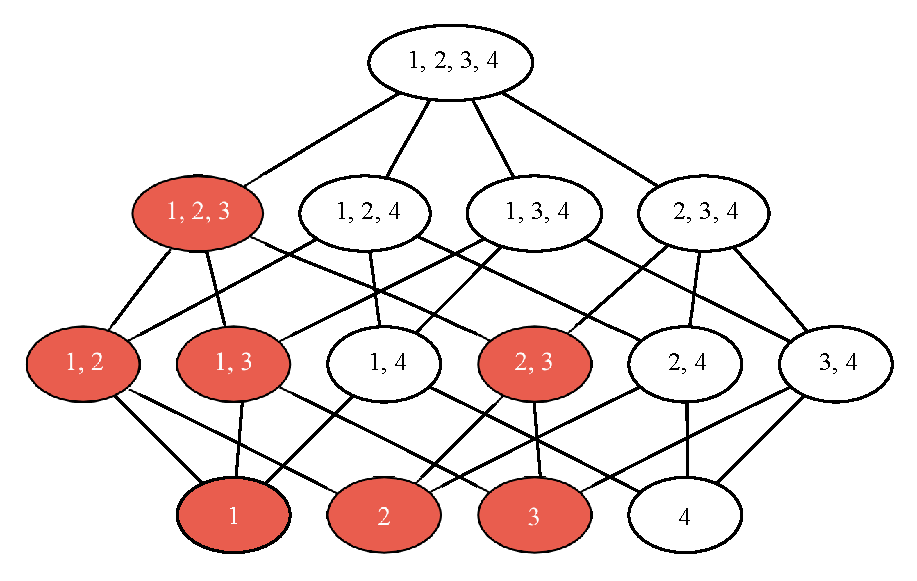
\includegraphics[]{res/downward.eps}
\end{figure}

%%%%%%%%%%%%%%%%%%
% Indien dit gekopieerd wordt, zie: https://en.wikibooks.org/wiki/LaTeX/Algorithms
%%%%%%%%%%%%%%%%%%
\begin{algorithm}
\caption{Pseudocode van Apriori, waarbij de frequente itemsets ontdekt worden.}
\label{algo:apriori}
\begin{algorithmic}
\Require T: Transactionset
\Function{apriori}{T}
    \State $C_1 \gets initialPass(T)$
    \Comment{Generating frequent 1-itemsets}
    \State $F_1 \gets \{f \mid f \in C_1 \wedge minsup \leq \frac{|f|}{|T|} \}$
    \State $k\gets 2$
    \While {$F_{k-1} \neq \emptyset$}
        \State $C_k \gets candidateGen(F_{k-1})$
        \For {$t \in T$} 
        \Comment{Iterate over all transactions}
            \For {$c \in C_{k} $}
                \If {$c \subseteq t$}
                    \State $|c|\gets |c| + 1$
                    \Comment{Increase count of candidate c}
                \EndIf
            \EndFor
        \EndFor
        \State $F_k \gets \{c\mid minsup \leq \frac{|c|}{|T|} \}$
        \State $k \gets k + 1$
    \EndWhile
    \State \Return $F \gets \cup_k F_k$ 
\EndFunction
\end{algorithmic}
\end{algorithm}

\newpage
Apriori past deze eigenschap toe door eerst de 1-item frequente itemsets te zoeken; door permutatie onstaan dan kandidaat-2-itemsets. Deze worden getest of ze voldoen aan de minimale \emph{support}. Indien dit het geval is, worden ze toegevoegd aan de frequente 2-itemset. Dit proces wordt iteratief herhaald tot alle frequente k-itemsets gevonden zijn.

Het genereren van de kandidaten wordt beschreven in algoritme \ref{algo:candidateGen}; de functie genereert een superset van frequente k-itemsets $ C_k \supseteq F_k$ op basis van de frequente itemsets $F_{k-1}$. Dit gebeurt in in twee stappen:

\begin{enumerate}
\item \textbf{Join}: Alle mogelijke kandidaat-k-itemsets $C_k$ worden gegenereerd op basis van $F_{k-1}$.
\item \textbf{Prune}: Kandidaten welke---door de \emph{downward closure property}---niet frequent kunnen zijn worden verwijderend uit $C_k$.
\end{enumerate}

Om de \emph{join}-stap te voltooien, worden kandidaat-k-itemsets beschreven volgens:

\begin{equation}
C_k \gets \{a \cup \{b\} \mid a \in F_{k-1} \wedge b \notin a \}
\end{equation}

De itemset $a$ is dus een element van de set van frequente-k-1-itemset, wat maakt dat $a$ zelf een frequente-k-1-itemset is. Bij deze itemset $a$ wordt een item $b$ toegevoegd, wat niet voorkomt in de itemset $a$. Hierdoor is een k-itemset ontstaan.

\begin{equation}
\{s \mid s \subset c \wedge |s| = k - 1\}
\end{equation}

De \emph{prune}-stap verwijdert alle subsets $s \subset c$ uit de kandidaten $c \in C_k$ die niet voorkwomen in de frequente itemset $F_{k-1}$. De subset $s$ moet voor deze reden $k-1$ items bevatten.

%%%%%%%%%%%%%%%%%%
% Indien dit gekopieerd wordt, zie: https://en.wikibooks.org/wiki/LaTeX/Algorithms
%%%%%%%%%%%%%%%%%%
\begin{algorithm}
\caption{Pseudocode om kandidaten te genereren uit frequente k-1-itemsets.}
\label{algo:candidateGen}
\begin{algorithmic} 
\Require $F_{k-1}$: Frequent k-1-itemset
\Function{candidateGen}{$F_{k-1}$}
    \State $C_k \gets \emptyset$
    \Comment{Starting with an empty set}
    \For {$C_k \gets \{a \cup \{b\} \mid a \subset F_{k-1} \wedge b \notin a \}$}
    	\Comment{Join}
        \For {$\{s \mid s \subset c \wedge |s| = k - 1\}$} 
        	\If {$s \notin F_{k-1}$}
            	\State $C_k \gets C_k - c$ 
                \Comment{Prune}
            \EndIf
        \EndFor
    \EndFor
    \State \Return $C_k$ 
\EndFunction
\end{algorithmic}
\end{algorithm}
%
Algoritme \ref{algo:apriori} is dus in staat alle frequente itemsets met een minimale \emph{support} $minsup$ te ontdekken, hieruit kunnen dan \emph{association rules} gedestilleerd worden. Dit gebeurt door voor iedere frequente itemset $F_k \in F$ iteratief iedere strikte subset $E \subset F_k$ te toetsen aan de minimale \emph{confidence} $minconf$.
%
%%%%%%%%%%%%%%%%%%
% Indien dit gekopieerd wordt, zie: https://en.wikibooks.org/wiki/LaTeX/Algorithms
%%%%%%%%%%%%%%%%%%
\begin{algorithm}
\caption{Pseudocode om \emph{asssociation rules} uit frequente itemsets te genereren.}
\label{algo:step_2}
\begin{algorithmic} 
\Require $F$: Set of frequent itemsets
\Function{rulesGen}{$F$}
    \For {$F_k \in F$}
        \For {$\{E \subset F_k| E \neq \emptyset \wedge E \neq F_k \}$} 
        	\If {$\conf\left(E \Rightarrow E \cap F_k \right) \geq minconf$}
            	\State Assocation rule $E \Rightarrow E \cap F_k$ found
            \EndIf
        \EndFor
    \EndFor
\EndFunction
\end{algorithmic}
\end{algorithm}
%
\subsection{Zeldzame itemprobleem}
In bepaalde datasets komen bepaalde items significant meer voor dan andere items. In het voorbeeld van de supermarkt zien we bijvoorbeeld terug in de wekelijkse aankoop van brood en de---hopelijk---eenmalige aankoop van een broodrooster. Het probleem is dus dat de minimaal benodigde \emph{support} voor ieder item hetzelfde is, onafhankelijk van de frequentie van dat item. De keuze van deze drempelwaarde heeft dus een twee gevolgen:

\begin{itemize}
\item \textbf{Minimale \emph{support} is hoog}: \emph{Association rules} met \emph{rare items} zullen niet gevonden worden.
\item \textbf{Minimale \emph{support} is laag}: Frequente items zullen met elkaar gecombineerd worden, wat ook minder betekenisvolle regels tot gevolg heeft. 
\end{itemize}

Door individuele items een \emph{minimum item support} MIS toe te kennen, wat we noteren als $\MIS\left(i\right)$, kan dit probleem opgelost worden. De \emph{support} dient dan groter te zijn dan de minimale MIS van itemset $X \cup Y = \{i_1, i_2, ..., i_r\} \textrm{ met } i_j \in I$.

\begin{equation}
\supp(X \cup Y) \geq \min\left(\MIS(i_1), \MIS(i_2), ..., \MIS(i_r) \right)
\end{equation}

Om te verhinderen dat frequente items samen met \emph{rare items} voorkomen, mag het verschil tussen de grootste en kleinste MIS niet groter zijn dan een bepaalde drempelwaarde. Dit wordt de \emph{support difference constraint} $\phi$ genoemd. 

\begin{equation}
\phi \geq \max_{i\in X \cup Y}\left(\supp(i) - \min_{i\in X \cup Y}\left(\supp(i)\right)\right)
\end{equation}

Wat vereenvoudigd kan worden tot:

\begin{equation}
\phi \geq \max_{i\in X \cup Y}\left(\supp(i)\right) - \min_{i\in X \cup Y}\left(\supp(i)\right)
\end{equation}

Door de introductie van \emph{minimum item supports} is de \emph{downward closure}-eigenschap niet meer geldig\cite{Liu1999MiningSupports}. Een alternatief hiervoor is \emph{sorted closure}; waarbij items gesorteerd worden volgens hun MIS. Dit valt echter buiten de scope van deze cursus.
%
\subsection{Class association rules}
Bij \emph{association mining} kunnen items voorkomen als een conditie $i \in X$ of als een consequentie $i \in Y$. Indien men echter enkel ge\"interesseerd is in de regels die een bepaalde consequentie opleveren, dan willen we alle \emph{class association rules} (CAR) met een klasse $y$ van de set van klasse-labels $Y$ vinden. Formeel wordt dit:

\begin{equation}
X \Rightarrow y \textrm{ met } X \subseteq I \textrm{ en } y \in Y
\end{equation}

Aangezien de klasse-labels al gekend zijn, is het vinden van frequente k-itemsets voldoende om de regels te genereren. Dit betekent dus dat Apriori aangepast kan worden voor CAR. 

Daarnaast is het ook nuttig om op te merken dat de gekende definities voor de \emph{support} en \emph{confidence} hetzelfde blijven.
%
\newpage
\begin{table}
\centering
\caption{Set van transacties $T$.}
\label{tabel:7-transacties}
\begin{tabular}{c|c|c}
\textbf{Doc} & \textbf{Dataset} & \textbf{Klasse} \\
1 & $\{student, leerkracht, school\}$ & $onderwijs$ \\
2 & $\{student, school\}$ & $onderwijs$ \\
3 & $\{leerkracht, school, stad, wedstrijd\}$ & $onderwijs$\\
4 & $\{basketball, lopen\}$ & $sport$ \\
5 & $\{basketball, speler, toeschouwer\}$ & $sport$\\
6 & $\{basketball, coach, wedstrijd, team\}$ & $sport$\\
7 & $\{basketball, team, stad, wedstrijd\}$ & $sport$
\end{tabular}
\end{table}
%
\paragraph{Voorbeeld}
Stel $minsup = 20\%$ en $minconf = 60\%$. We beschouwen de dataset in tabel \ref{tabel:7-transacties}, welke bestaat uit enkele frequente woorden van documenten die geclassificeerd zijn als \emph{sport} of \emph{onderwijs}.

\begin{table}
\centering
\caption{Ontdekte regels uit de transacties opgesomd in tabel \ref{tabel:7-transacties}.}
\label{tabel:regels-7-transacties}
\begin{tabular}{c|c|c}
\textbf{Regel} & \textbf{supp} & \textbf{conf} \\
$\{student, school\} \Rightarrow onderwijs$ & $\dfrac{2}{7}=29\%$ & $\dfrac{2}{2}=100\%$\\[10pt]
$\{basketball\} \Rightarrow sport$ & $\dfrac{4}{7}=57\%$ & $\dfrac{4}{4}=100\%$\\[10pt]
$\{wedstrijd\} \Rightarrow sport$ & $\dfrac{2}{7}=29\%$ & $\dfrac{2}{3}=67\%$ \\[10pt]
$\{team\} \Rightarrow sport$ & $\dfrac{2}{7}=29\%$ & $\dfrac{2}{2}=100\%$ \\[10pt]
$\{basketball, wedstrijd\} \Rightarrow sport$ & $\dfrac{2}{7}=29\%$ & $\dfrac{2}{2}=100\%$\\[10pt]
$\{basketball, team\} \Rightarrow sport$ & $\dfrac{2}{7}=29\%$ & $\dfrac{2}{2}=100\%$\\[10pt]
$\{team, wedstrijd\} \Rightarrow sport$ & $\dfrac{2}{7}=29\%$ & $\dfrac{2}{2}=100\%$\\[10pt]
$\{basketball, wedstrijd, team\} \Rightarrow sport$ & $\dfrac{2}{7}=29\%$ & $\dfrac{2}{2}=100\%$\\

\end{tabular}
\end{table}

%
\section{Sequenti\"ele patronen}
Een limitatie van voorgaande \emph{association rules} is dat er geen rekening gehouden wordt met de volgorde van transacties. Het kan echter wel nuttig zijn om deze volgorde in beschouwing te nemen, wat leidt tot sequenties. Men defini\"eert een sequentie $s$ als een \textbf{geordende} lijst van itemsets $a_i$. Een k-sequentie is een sequentie van k itemsets; wat gelijkaardig is aan k-itemsets.

\begin{equation}
s = \langle a_1, a_2, a_3, ..., a_r \mid a \subseteq I  \rangle
\end{equation}

\paragraph{sub- en supersequenties}
Indien we twee sequenties $s_1 = \langle a_1, ..., a_r \rangle
$ en $s_2 = \langle b_1, ..., b_v \rangle$ beschouwen, dan kunnen we stellen dat sequentie $s_1$ een \emph{subsequentie} is van sequentie $s_2$ als iedere itemset ook een deelverzameling is. 
\begin{equation}
s_1 \subseteq s_2 \iff \{a_i \subseteq b_i \mid \{i \in \langle\mathds{Z}^{+}\rangle \mid i \leq r \} \} 
\end{equation}

\subsection{Mining algoritmes}
Om sequenties te \emph{minen}, kan het \emph{Generalized Sequential Pattern} of kortweg GSP-algoritme gebruikt worden. Dit algoritme lijkt zeer sterk op Apriori---wat bij algoritme \ref{algo:apriori} is besproken. Wat wel verschilt is de generatie van kandidaten. De twee stappen (\emph{join} en \emph{prune}) van Apriori komen ook wel weer terug:

\begin{enumerate}
\item \textbf{Join}: Alle mogelijke kandidaat-k-sequenties worden gegenereerd door $F_{k-1}$ te \emph{joinen} met $F_{k-1}$. De volledige sequentie $s_1$ \emph{joint} de volledige sequentie $s_2$ als de subsequentie van $s_1$ zonder het eerste item gelijk is aan de subsequentie van $s_2$ zonder het laatste item. 

Afhankelijk of het laatste element van $s_2$ een aparte set vormt, zijn er twee gevallen: 
\begin{enumerate}
\item Het item vormt een aparte set op het einde van $s_1$ als het ook een aparte set vormde in $s_2$.
\item Het item wordt aan het laatste element van $s_1$ toegevoegd indien het geen aparte set vormde in $s_2$.
\end{enumerate}

Het \emph{joinen} van $F_1$ met $F_1$ is ook bijzonder, aangezien er hier nog geen itemsets zijn ($k=1$). Dus wordt het item van $s_2$ zowel als itemset als apart element toegevoegd.
\item \textbf{Prune}: Kandidaten waarbij een van de k-1-subsequenties niet frequent is, worden verwijderd.
\end{enumerate}

\paragraph{Voorbeeld} In tabel \ref{tabel:candidates-3-sequences} wordt de generatie van kandidaten uitgewerkt. Indien we we het algoritme overlopen en stellen dat $s_1 = \langle \{1,2\}\{4\}\rangle $, dan is de subsequentie zonder het eerste item $\langle \{2\}\{4\}\rangle $. Dit komt overeen met de laatste twee frequente-3-sequenties. Deze worden dan gecombineerd, rekening houdende met de bovengestelde voorwaarde. 

\begin{table}
\centering
\caption{Kandidaten uit frequente-3-sequenties.}
\label{tabel:candidates-3-sequences}
\begin{tabular}{c|c|c}
\textbf{Frequente-3-}& \multicolumn{2}{c}{\textbf{Kandidaat-4-sequenties}} \\
\textbf{sequenties} & \textbf{Na \emph{join}} & \textbf{Na \emph{prune}} \\
$ \langle \{1,2\}\{4\}\rangle $ & $ \langle \{1,2\}\{4,5\}\rangle $ & $\langle \{1,2\}\{4,5\}\rangle $ \\ 
$ \langle \{1,2\}\{5\}\rangle $ & $ \langle \{1,2\}\{4\}\{6\}\rangle $ & \\ 
$ \langle \{1\}\{4,5\}\rangle $ &  & \\ 
$ \langle \{1,4\}\{6\}\rangle $ &  & \\ 
$ \langle \{2\}\{4,5\}\rangle $ &  & \\ 
$\langle\{2\}\{4\}\{6\}\rangle$ &  & \\ 


\end{tabular}
\end{table}
%
%Chapter 3: An introduction to R: Association rules
\chapter{De R programmeertaal}
\section{Wat is R}
\marginnote{R is beschikbaar op \url{https://www.r-project.com} en RStudio is verkrijgbaar op \url{https://www.rstudio.com}}
R is een scriptingtaal speciaal ontwikkeld voor het gebruik in statistische software. De taal is open source en dus vrij beschikbaar. Er is ook een gratis IDE beschikbaar. De grote kracht van deze taal is de grote hoeveelheid beschikbare packages waarbij gebruikers reeds algoritmen ge\"implementeerd hebben. Zo kan de gebruiker van de taal dus focussen op zijn specifiek probleem, zonder noodzakelijk bezig te zijn met details.
\section{Basisconcepten}
\subsection{Variabelen}
Omdat R een dynamische taal is, is het niet nodig om het type te vermelden. Men kan variabelen op 2 manieren toewijzen:
\begin{minted}{R}
x = 123
y <- 321
z = "Dit is een test string"
\end{minted}
Merk op dat indien statements op 1 lijn staan er geen puntkomma's nodig zijn om deze af te sluiten. R heeft heel wat functies al ingebouwd. Voorbeelden hiervan zijn \mintinline{R}{sqrt(x),cos(x),log(x)} en veel meer. Verder volgt R ook dezelfde commando's als op Unix systemen. Indien een gebruiker dus een variable wil verwijderen uit de workspace kan met \mintinline{R}{rm(x)} gebruiken. Gelijkaardig kan men \mintinline{R}{ls()} gebruiken. Indien men RStudio gebruikt als IDE dan staan de variabelen automatisch rechts vermeld.

Bij \emph{data mining} en statistiek maakt men vaak gebruik van vectoren en matrices om data voor te stellen. Het is daarom ook logisch dat R heel wat methoden bevat om matrices en vectoren te manipuleren. Hieronder zijn enkel voorbeelden gegeven.
\newpage
\subsection{Voorbeeldcode: vectoren en matrices}
\begin{minted}{R}
#Comments beginnen met een #-teken.
#Het alloceren van een vector
positie <- c(0,5,0)
#Het is ook mogelijk om automatisch een vector op te vullen
sequence <- seq(from=0, to=10, by=1) #sequence = {0,1,2,3,4,5,6,7,8,9,10}
#Of om een bepaalde herhaling uit te voeren
rep = rep(2, times=5) #rep = {2, 2}, 2 kan ook een vector zijn
#Optellen van 2 vectoren
delta_pos <- {1,0,0}
positie = positie + delta_pos
#constanten en een vector:
positie = positie * 0.5
#Vectoren in R beginnen, in tegenstelling tot veel andere talen, bij 1:
first_element = sequence[1]
last_element = sequence[11]
#Alles behalve 1 element:
all_without_first = sequence[-1]
#Subset:
first_five = sequence[1:5]
#Matrices
mat = matrix(1:9, nrow=3, byrow=TRUE) #Vult de matrix met waarden per rij( dus rij 1: 1,2,3 )
mat = matrix(1:9, nrow=3, byrow=FALSE) #Vult de matrix met waarden per kolom( dus rij 1: 1,4,7 )
#Matrices indexering:
top_left = mat[1,1] #top_left = 1
row_two = mat[2,] #row_to = {2,5,8}
\end{minted}
\subsection{Controle structuren}
R heeft dezelfde controlestructuren zoals men aantreft in andere programmeertalen. Deze zijn:
\begin{itemize}
\item \textbf{if}: \mintinline{R}{ if(condition) expr1 else expr2 } Hierbij kan men braces gebruiken indien de expressies uit meerdere statements bestaan. 
\item \textbf{for}: \mintinline{R}{ for( var in seq ) expr }
\item \textbf{while}: \mintinline{R}{ while( cond ) expr }
\item \textbf{switch}: \mintinline{R}{ switch( expr, case1, case2, .. ) }
\end{itemize}
\newpage
\subsection{Methoden}
Methoden in R worden als volgt gedefinieerd en opgeroepen: 
\begin{minted}{R}
mean <- function( input )
{
	return( sum( input ) / length( input ) )
}
mean( c( 5, 10 ) ) #print 7.5 uit
\end{minted}
\subsection{Dataframes}
Een andere vaak gebruikte datastructuur is een \emph{dataframe}. Deze structuur wordt het best vergeleken met een matrix. Het bestaat uit een collectie lijsten met dezelfde lengte. Een voordeel aan dataframes vergeleken met matrices is dat ze gebruikt kunnen worden  zoals een database. De gebruiker kan rijen toevoegen of een query uitvoeren op een bepaalde kolom. Men kan een dataframe bekijken via \mintinline{R}{View(dataframe)}. Vectoren toevoegen doet met via \mintinline{R}{attach() en detach()}. Bepaalde data opvragen kan als volgt: \mintinline{R}{data[ gender=="male" & age > 18,]}. Let hierbij op de komma om alle kolommen te selecteren.
%
\section{Het gebruik van packages}
\marginnote{Een overzicht van alle packages is beschikbaar op: \url{https://cran.r-project.org/web/packages/available_packages_by_date.html}}
De grote sterkte van R zijn de grote hoeveelheid aanwezige \emph{packages}, bibliotheken met een bepaald doel. Het installeren van deze \emph{packages} is zeer eenvoudig: \mintinline{R}{install.packages(wordcloud)}. en het gebruik nog eenvoudiger: \mintinline{R}{library(wordcloud)}. Een \emph{package} moet maar eenmaal ge\"installeerd worden en kan daarna met bovenstaand commando geladen worden.
%
\section{Association rules in R}
Als concreet voorbeeld nemen we de \emph{association rules} aangeleerd in vorig hoofdstuk. Hiervoor is het package \mintinline{R}{arules} beschikbaar.
Stel dat we volgend bestand beschikbaar hebben:
\marginnote{De inhoud van het testbestand: transactions.txt}
\begin{minted}{R}
A,B,C
B,C
A,B,D
A,B,C,D
A,B
B,C
A
B
\end{minted}
Het inlezen is zeer eenvoudig:
\begin{minted}{R}
transactions <- read.transactions("transactions", format="basket", sep=",")
\end{minted}
Hier geven we de bestandsnaam mee, samen met het formaat: een \emph{basket}. Dit maakt het duidelijk voor het package dat de data een winkelmand voorstelt. Tot slot vermelden we de seperator waarmee de data gescheiden is.

Indien we de transactions willen bekijken dan kan dit via een aantal methoden: \mintinline{R}{inspect(transactions)} print de data uit in de console, \mintinline{R}{image(transactions)} geeft een afbeelding van een grid weer waarbij een cel zwart is ingekleurd indien een item aanwezig is en \mintinline{R}{itemFrequencyPlot(transactions, support=0.1)} visualiseert hoe vaak elk item voorkomt.

In het vorig hoofdstuk hebben het apriori algoritme besproken. Ook dit algoritme is aanwezig in deze \emph{package}. We kunnen automatisch de regels laten genereren via:
\begin{minted}{R}
rules <- apriori(transactions, paramater=list(supp=0.5,conf=0.5))
inspect( rules )
\end{minted}
Dan krijgen we de volgende output:
\begin{minted}{console}
> inspect(rules)
    lhs    rhs support confidence lift     
[1] {}  => {C} 0.500   0.5000000  1.0000000
[2] {}  => {A} 0.625   0.6250000  1.0000000
[3] {}  => {B} 0.875   0.8750000  1.0000000
[4] {C} => {B} 0.500   1.0000000  1.1428571
[5] {B} => {C} 0.500   0.5714286  1.1428571
[6] {A} => {B} 0.500   0.8000000  0.9142857
[7] {B} => {A} 0.500   0.5714286  0.9142857
\end{minted}

We kunnen ook sequenti\"ele patronen laten genereren via het \mintinline{R}{arulesSequences} package. 
%
%Chapter 4: Unsupervised learning & clustering
\chapter{Unsupervised learning \& clustering}
\section{Introductie}
Algemeen gezien bouwen \emph{machine learning}-technieken een model op basis van een (voorbeeld)-dataset; waarbij het doel is om een structuur die in de dataset zit naar boven te brengen. Het kan zijn dat deze structuur al aangeduid wordt doordat de data gelabeld is, in dit geval spreken we van \emph{supervised learning}. Indien de data nog niet gelabeld is, dient een \emph{unsupervised learning}-techniek gebruikt te worden.

\section{Clustering}
\emph{Clustering} is een typische \emph{unsupervised learning}-techniek, waarbij \emph{similarity groups} of clusters worden gezocht. Dit zijn data-elementen welke (per cluster) onderling sterk op elkaar gelijken. De data is dus nog niet geclassificeerd; er zijn geen labels voorzien. 

Om elementen met elkaar te kunnen vergelijken is een \emph{distance}-functie nodig. Door te clusteren dienen dan twee parameters geoptimaliseerd te worden:

\begin{itemize}
\item \textbf{Interclusterafstand}: De afstand tussen elementen van verschillende clusters dient maximaal te zijn. 
\item \textbf{Intraclusterafstand}: De afstand tussen elementen van eenzelfde cluster dient minimaal te zijn.
\end{itemize}

Het spreekt voor zich dat deze parameters een maatstaaf zijn voor de kwaliteit van het resultaat. De \emph{distance}-functie heeft een invloed op dit resultaat, alsook het algoritme zelf. Ook speelt het mee hoe de clusters gevormd zijn.
%
\begin{figure}[h]
\centering
\caption{Een voorbeeld van 6 elementen die met een hi\"erarchisch clusteringsalgoritme gegroepeerd zijn. }
\label{figure:hierarchical_clustering}
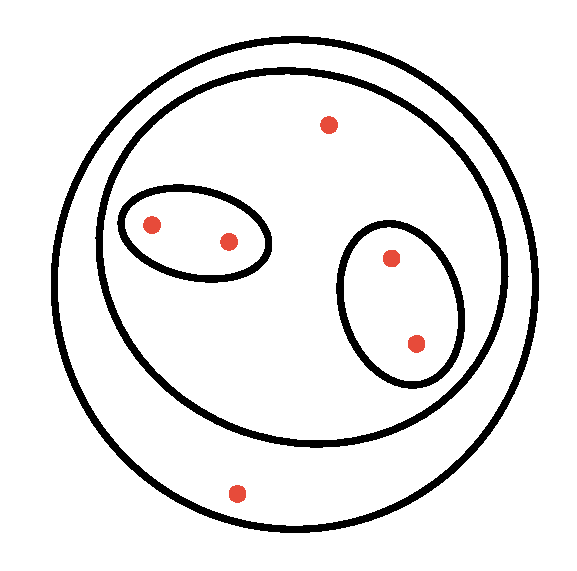
\includegraphics[width=0.40\textwidth]{res/ch4_hierarchical_clustering.eps}
\end{figure}
%
Wat algoritmes betreft, beschouwt men meestal twee soorten algoritmes. De eerste groep zijn de \emph{partitional clustering}-algoritmes, waar K-means onder valt. Hierbij wordt een groep elementen onderverdeeld in niet-overlappende subsets. \emph{Hierarchical clustering} is de tweede soort, waarbij een boomstructuur van geneste clusters wordt opgebouwd.  
%
\subsection{K-means}
Zoals eerder vermeld, is K-means een \emph{partitional clustering}-algoritme. De data wordt dus verdeeld in $k$ niet-overlappende clusters. Deze parameter $k$ wordt door de gebruiker opgegeven.

De data $D$ is een set van $r$ punten in een $n$-dimensionale vectorruimte. 

\begin{equation}
D= \{x_1, \dots, x_r \mid x_i \in \mathds{R}^n\}
\end{equation}

Elke cluster heeft een \emph{centroid}, een punt in het midden van de cluster. Bij de start van het algoritme worden $k$ punten random aangeduid als \emph{centroid}. Ieder punt wordt daarna een aan cluster toegewezen, afhankelijk van de afstand tot de \emph{centroid}. Hierna worden de \emph{centroids} herberekend, op basis van de huidige clusters. Dit wordt herhaald tot er geen convergentie meer waargenomen wordt. 

%%%%%%%%%%%%%%%%%%
% Indien dit gekopieerd wordt, zie: https://en.wikibooks.org/wiki/LaTeX/Algorithms
%%%%%%%%%%%%%%%%%%
\begin{algorithm}
\caption{Pseudocode voor het K-means-algoritme.}
\label{algo:kmeans}
\begin{algorithmic} 
\Require $k$: Number of clusters
\Require $D$: Data
\Function{k-means}{$k$,$D$}
    \State $C \gets randomSelection(k, D)$
    \Comment{Random centroids $C$}
    \Repeat
    \For {$x\in D$}
    	\For {$m \in C$}
        	\State compute distance from $x$ to $m$
        \EndFor
        \State assign $x$ to closest centroid $m$
    \EndFor
    \State $C \gets recomputeCentroids$
    \Until{stopping criterion is met}
    \State \Return $C$ 
\EndFunction
\end{algorithmic}
\end{algorithm}

Het \emph{stopping criterion} in algoritme \ref{algo:kmeans} kan op meerdere manieren ge\"implementeerd worden. Enkele mogelijkheden zijn:

\begin{enumerate}
\item Geen of weinig toekenningen van datapunten aan andere clusters.
\item Geen of minimale verandering van de \emph{centroids}.
\item Minimale afname in de \emph{sum of squared error}. Hierbij wordt per cluster $C_i$  de afstand $d$ tussen ieder punt $x \in C_i$ en de \emph{centroid} $m_i$ berekend.
\begin{equation}
SSE = \sum_{j=1}^k{\sum_{x\in C_i}{d\left( x, m_i \right)^2}}
\end{equation}
\end{enumerate}

\begin{figure}
\centering
\caption{Een voorbeeld van een gegenereerde tweedimensionale dataset, welke opgedeeld is in drie clusters van gelijke grootte.}
\label{figure:clusters}
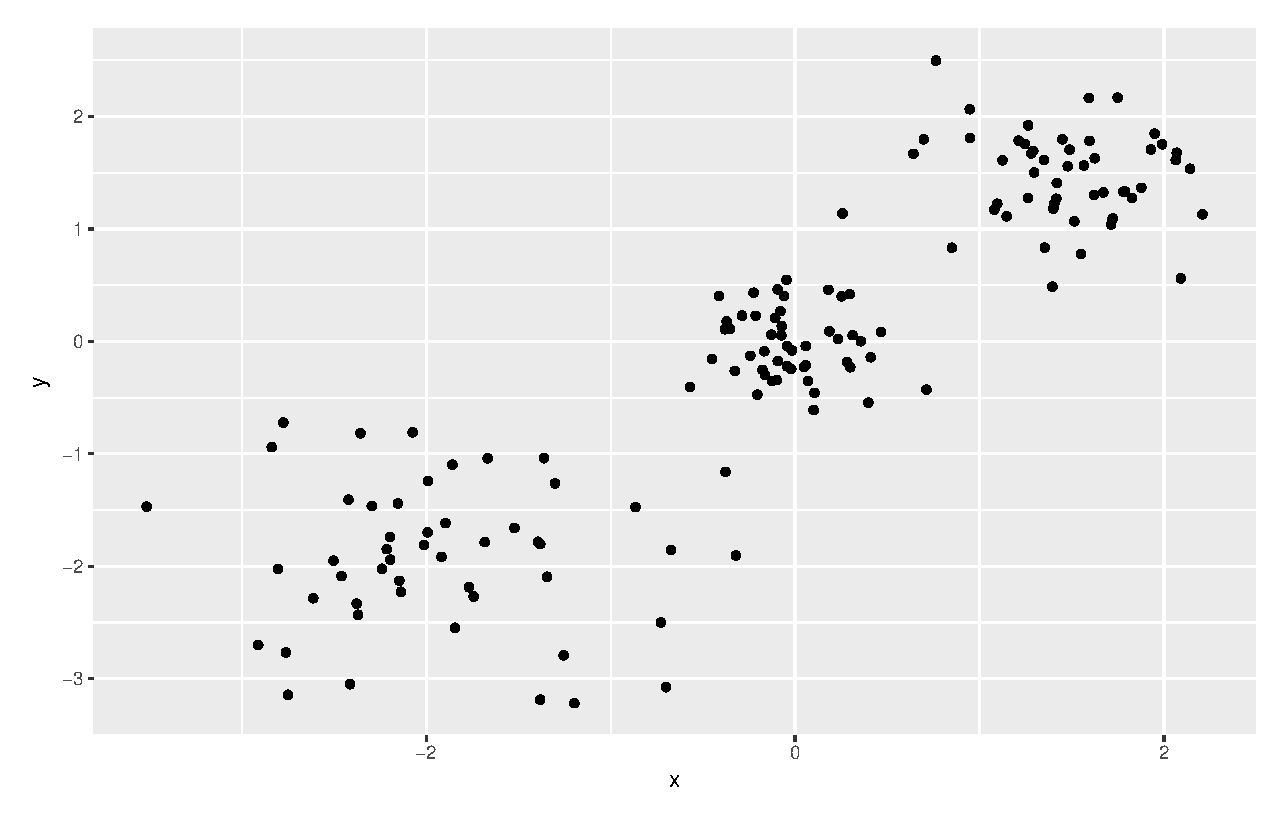
\includegraphics[width=\textwidth]{res/ch4_kmeans_before.eps}
\end{figure}

\begin{figure}
\centering
\caption{Op de dataset van figuur \ref{figure:clusters} is het \emph{K-means}-algoritme toegepast. De code voor het genereren van deze dataset en het clusteren staat op Github.}
\label{figure:clusters_kmeans}
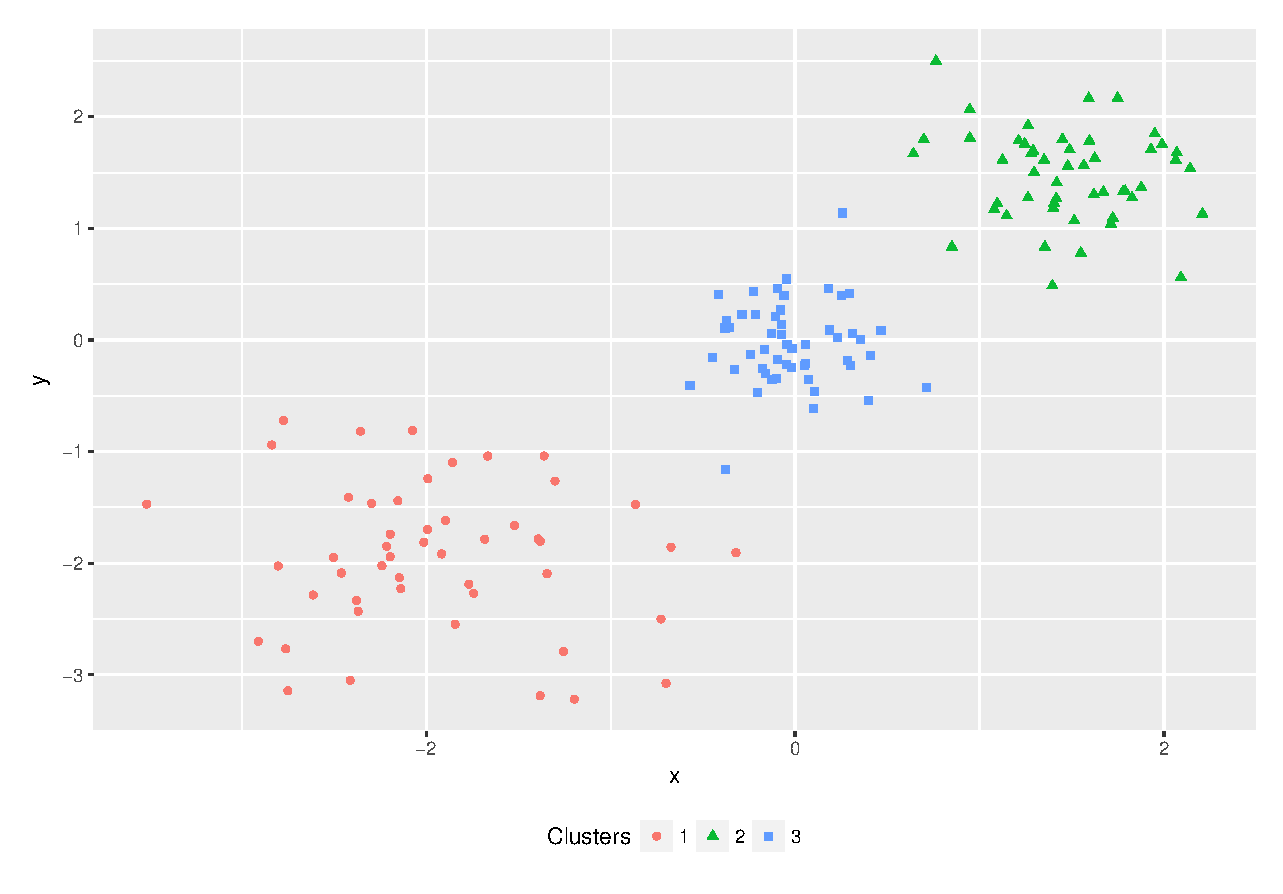
\includegraphics[width=\textwidth]{res/ch4_kmeans_after.eps}
\end{figure}

\paragraph{Distance functions}
In een Euclidische vectorruimte $\mathds{R}^n$ kan de afstandsfunctie $d$ op een volgende manier beschreven worden:

\begin{equation}
d(x,m)=||x-m||=\sqrt[]{\left(x_1-m_1\right)^2+\dots+\left(x_n-m_n\right)^2}
\end{equation}

Voor de \emph{centroids} is het dan mogelijk om het gemiddelde te gebruiken, wat per cluster $C_i$ tot de volgende formule leidt:

\begin{equation}
m_i^{t} = \frac{1}{|C_i^{t-1}|}\cdot \sum_{x\in C_i^{t-1}}{x}
\end{equation}

%
\paragraph{Voor- en nadelen}
Het K-means-algoritme is vrij eenvoudig om te begrijpen en te implementeren. Daarnaast is het ook nog behoorlijk effici\"ent, met een tijdscomplexiteit $O\left(k\cdot n \cdot i \cdot r \right)$ met $i$ iteraties \cite{jin2011k}. Er wordt ook veel werk gestoken in een paralleliseerbare versie \cite{zhao2009parallel}. Dit alles maakt dat K-means het populairste clusterings-algoritme is.

Er zijn echter ook nadelen aan het algoritme; waarvan de volgende het meest noemenswaardig zijn. 

\begin{itemize}
\item Het gemiddelde van een cluster dient gedefini\"eerd te zijn. 
\item Het algoritme is gevoelig voor initi\"ele \emph{centroids}; dit is ge\"ilustreerd in figuur \ref{figure:clusters_kmeans_wrong_seed}. Door meerdere \emph{passes} te doen, kan dit probleem verholpen worden. Daarnaast zijn er ook methoden om goede \emph{seeds} te kiezen voor de initi\"ele \emph{centroids}.

\begin{figure}
\centering
\caption{Dezelfde dataset van \ref{figure:clusters}, maar met ongelukkig gekozen \emph{centroids}. Merk op dat er nog steeds 3 clusters zijn, maar dat dit niet het globale optimum heeft gelokaliseerd. }
\label{figure:clusters_kmeans_wrong_seed}
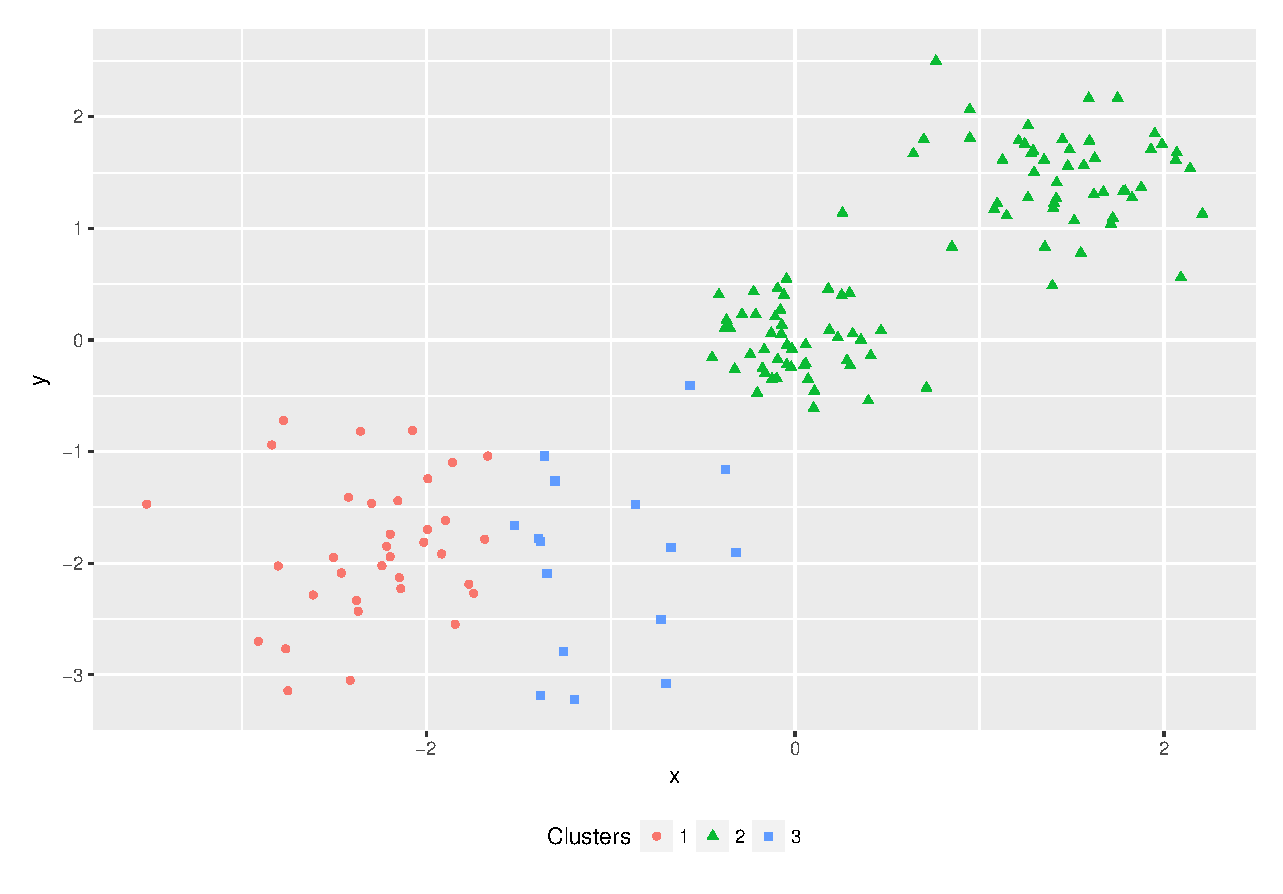
\includegraphics[width=\textwidth]{res/ch4_kmeans_wrong_seed.eps}
\end{figure}

\item De gebruiker dient zelf het aantal clusters $k$ op te geven.
\item Het algoritme is gevoelig voor \emph{outliers}. Dit kan opgelost worden door deze punten na enkele iteraties te verwijderen of door te clusteren op een random geselecteerde subset van de data. Dit verkleint de kans dat een \emph{outlier} geselecteerd wordt. 
\item K-means is enkel bruikbaar voor hyper-ellipso\"iden.


\begin{figure}
\centering
\caption{Een spiraalvormige dataset; nog steeds met 3 clusters. K-means is niet in staat de clusters correct te classificeren. De code hiervoor staat op Github.}
\label{figure:clusters_kmeans_spiral}
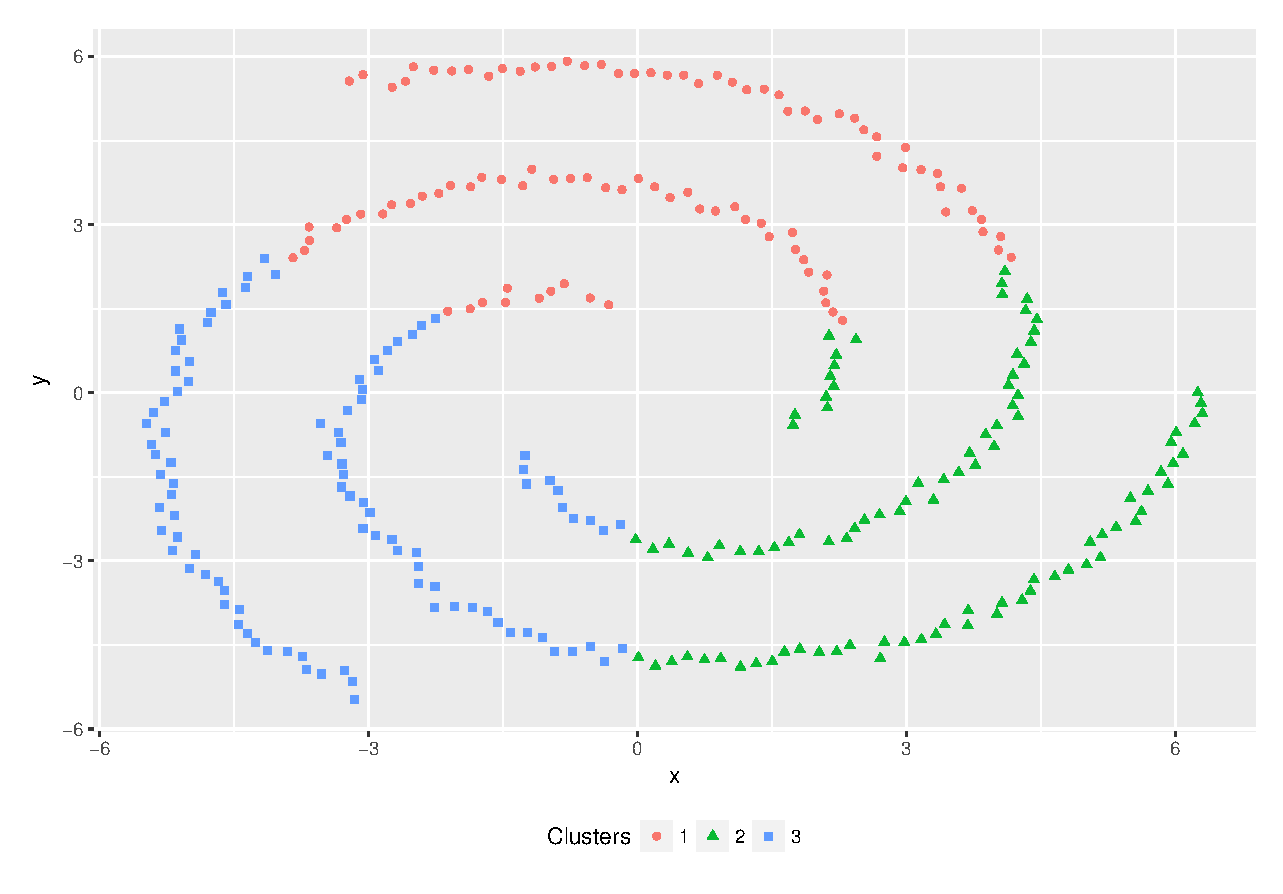
\includegraphics[width=\textwidth]{res/ch4_kmeans_spiral.eps}
\end{figure}
\end{itemize}

%
%Chapter 5: Supervised learning
\chapter{Supervised learning}
\section{Introductie}
In tegenstelling tot bij \emph{unsupervised learning} beschikken we bij \emph{supervised learning} over een dataset waarbij het gewenste resultaat al bijgevoegd is. Deze dataset wordt ook nog eens opgedeeld in twee delen: Een eerste deel waarmee het algoritme bijleert, en een tweede om de nauwkeurigheid van het algoritme te testen. Merk op dat indien de tweede dataset ook gebruikt zou worden om het algoritme te trainen, dit geen goed beeld zou geven van de werking. 

\paragraph{Voorbeeld}
Een eerste voorbeeld waarop dit mogelijk is, is een creditcardmaatschappij. Stel dat een nieuwe klant een aanvraag indient om een creditcard te krijgen. Dan moet het bedrijf verschillende parameters analyseren zoals de leeftijd, of de persoon getrouwd is, het loon, welke leningen er al aanwezig zijn, \dots Het resultaat van de aanvraag is dan binair: wordt de aanvraag aanvaard of niet? 

\paragraph{Voorbeeld}
Een tweede voorbeeld is in een ziekenhuis. Hierbij moet er opnieuw aan de hand van een aantal parameters beslist worden of een pati\"ent opgenomen moet worden op intensive care. Aangezien dit een duur proces is, wensen ziekenhuizen dit enkel te doen voor pati\"enten met een hoog risico.

Algemeen heeft met dus een probleem met een aantal (discrete) uitkomsten. Hiervoor ontwikkelen we een oplossing waarbij een functie getraind wordt met een bestaande dataset. Dit wordt ook vaak \emph{classification} of \emph{inductive learning} genoemd.
\section{Voorbeeld en terminologie}
De data wordt gedefinieerd als een set van $k$ attributen: ${A_1, A_2,..,A_k}$. Elke rij heeft ook een label met een reeds gedefinieerde klasse. Hiervan komt de naam \emph{supervised}, we beschikken over leermateriaal. Het doel is om deze gegevens te gebruiken om een model zo te trainen dat een toekomstige rij, waarbij alle attributen aanwezig zijn, een correct label toe te kennen.
Na de training kan de data getest worden op een tweede dataset. Deze dataset bestaat uit een aantal rijen waarvan de klasse reeds bekend is. Met kan de \emph{accuracy} van het model dan als volgt berekenen:

\begin{equation}
\textrm{Correctheid} = \frac{\textrm{juiste gevallen}}{\textrm{totaal aantal testcases}}
\end{equation}

Algemeen volgen we dus dit patroon:

\begin{equation}
\textrm{Training data} \rightarrow \textrm{Learning  algoritm} \rightarrow \textrm{Model} \rightarrow \textrm{Test data} \rightarrow \textrm{Accuracy}
\end{equation}

Het is belangrijk om zich het doel te blijven herinneren tijdens dit proces. Stel in het voorbeeld van het creditcardmaatschappij dat we gewoon steeds \emph{geaccepteerd}  antwoorden. Dan zullen we dus een \emph{accuracy} van 50\% hebben. Het doel van het supervised learning algoritme is dus om (veel) beter te doen dan de reeds gebruikte methode.

Het aanleren wordt dus als volgt gedefinieerd. Stel dat we een dataset \emph{D} hebben met een taak \emph{T} en een manier om de kwaliteit te meten \emph{M}. Een computersysteem leert dan van \emph{D} om taak \emph{T} uit te voeren, indien na het leren het systeem beter presteert als het taak \emph{T} uitvoert. Dit wordt gemeten via \emph{M}.

Er is dus een cruciaal concept waar we steeds rekening mee moeten houden indien we gebruik maken van \emph{supervised learning}: De test- en trainingsdata moet voldoende representatief zijn voor de data die men in het echt zal krijgen.
\section{Decision trees}
Een eerste, simpele maar toch effici\"ente vorm van supervised learning zijn \emph{decision trees}. Deze beslissingsbomen werken volgens een simpel principe. Bovenaan de boom staat een eerste attribuut. Vanuit deze knoop vertrekken verbindingen naar andere knopen. Elke verbinding stelt een waarde van het attribuut voor.

\begin{figure}[h]
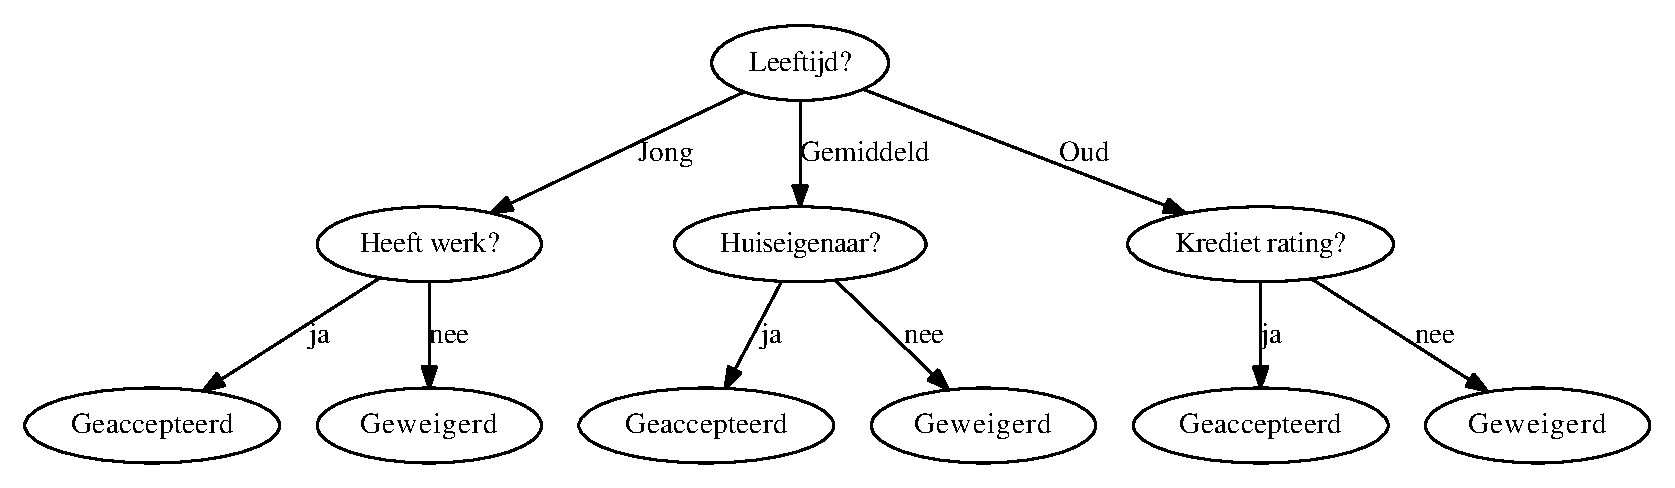
\includegraphics[width=\textwidth]{res/1}
\caption{Een voorbeeld van een beslissingsboom voor een creditcardmaatschappij.}
\label{fig:vb1_dt}
\end{figure}

Deze boom is afhankelijk van de gegeven data en is niet uniek, noch optimaal. Er bestaat een kleinere boom die dezelfde info geeft in minder nodes. We moeten dus proberen een zo klein mogelijk boom te construeren. Dit is echter geen triviale opgave en alle huidige algoritmes geven een benadering.

De boom kan worden omgezet naar een serie regels. Elk pad van de beginknoop tot aan een blad is een regel. Voor figuur ~\ref{fig:vb1_dt} geeft dit dus volgende regels:
\begin{itemize}
\item Leeftijd = jong, heeft werk? = ja $\Rightarrow$ Class = Geaccepteerd
\item Leeftijd = jong, heeft werk? = nee $\Rightarrow$ Class = Geweigerd
\item ...
\end{itemize}
Elk van deze regels heeft dan ook een \emph{support} en \emph{confidence} afhankelijk van de gebruikte dataset.

\subsection{Een simpel algoritme}
Een mogelijk algoritme is een \emph{divide-and-conquer} algoritme. 
%%%%%%%%%%%%%%%%%%
% Indien dit gekopieerd wordt, zie: https://en.wikibooks.org/wiki/LaTeX/Algorithms
%%%%%%%%%%%%%%%%%%
\begin{algorithm}
\caption{Voorbeeld van een beslissingsboom constructie algoritme}
\begin{algorithmic}[1]
\Require D: Training data, A: Attributen, T: Een knoop van de boom, C: De verzameling van klassen
\Function{maakBeslissingsBoom}{D,A,T}
\If {$D$ bevat enkel data van een bepaalde klasse $c_j \in C $}
    \State maak $T$ een blad met klasse $c_j$;
\ElsIf{ $A = \emptyset$ }
	\State Maak van $T$ een blad met het label van klasse $c_j$,
    \State waarbij $c_j$ de meest voorkomende klasse in $D$ is.;
\Else
	\State // $D$ bevat een mix van klassen.We selecteren een 
	\State // attribuut om $D$ verder te verdelen in subsets 
	\State // zodat elke subset minder onzuiverheden bevat.
    \State $p_0 = $ puriteitEval($D$)
    \For{ $A_i \in \{A_1, A_2, ..., A_k\} $ }
    	\State $p_i$ = puriteitsEval($A_i,D$); 
    \EndFor
    \State Selecteer $A_g \in \{A_1, A_2, ..., A_k\} $ met de minste puurheid,
    \State berekend met $p_0 - p_i$;
    \If{ $p_0 - p_g < drempelwaarde$ }
    	\State Maak van $T$ een blad met label $c_j$;
    \Else
    	\State Maak van T een beslissingsknoop voor $A_g$;
		\State Verdeel $D$ dan in $m$ sets $D_1, D_2, ..., D_m$ gebaseerd op 
        \State $A_g$, met de mogelijke waarden: $\{v_1,v_2,..v_m\}$ 
        \For{ $D_j$ in $\{D_1,D_2,..D_m\}$ }
        	\If{ $D_j \neq \emptyset $ }
            	\State Maak een tak $T_j$ voor $v_j$ als kind van $T$.
                \State decisionTree( $D_j, A-\{A_g\}, T_j$ )
            \EndIf
        \EndFor
    \EndIf
\EndIf
\EndFunction
\end{algorithmic}
\end{algorithm}

Bij dit algoritme nemen we aan dat alle data categorisch is. De boom wordt op een \emph{top-down} recursieve manier opgesteld. Dit wil zeggen dat we beginnen bij de bovenste knoop van de boom en zo verder afdalen tot de bladen gevormd zijn. Elementen uit de dataset worden verder onderverdeeld gebaseerd op hun attributen.

Het bovenste algoritme heeft enkele voorwaarden op te stoppen:

\begin{itemize}
\item Indien er geen elementen meer over zijn
\item Er zijn geen attributen meer die onderverdeeld moeten worden
\item Alle elementen bij een knoop behoren tot dezelfde klasse
\end{itemize}

De sleutel tot succes bij dit algoritme is de keuze van het attribuut om een tak te maken. Het doel is om de data zo puur mogelijk te maken: Een subset van data wordt als puur aanzien indien alle data tot dezelfde klasse behoort. Voor we verder ingaan op het maken van deze keuze moeten we eerst begrijpen wat puurheid nu eigenlijk is. We verklaren dit aan de hand van \emph{informatietheorie}.

\subsection{Informatietheorie}
Informatietheorie is een onderdeel van de wiskunde dat zich bezig houdt de opslag en verwerking van informatie. Het levert ons een basis om de inhoud van data te beschrijven. Een manier om dit beter te begrijpen is om dit voor te stellen als een antwoord op een vraag: Zal mijn worp kop of munt zijn? Indien men op voorhand al info heeft, men weet bijvoorbeeld dat de munt vervalst is, dan is het antwoord op de vraag minder relevant. Indien men dit nog niet weet, dan zou extra kennis dus welkom zijn. Het antwoord heeft dus een grotere waarde.

Informatietheorie gebruikt ditzelfde concept, maar gebruikt geen geld om de waarde van informatie uit te drukken, maar \emph{bits}. Een bit is net genoeg info om het antwoord te geven op een ja/neen vraag waarover men geen idee heeft, zoals het opwerpen van een munt.

Een belangrijke manier om hoeveelheden informatie uit te drukken is entropie. Entropie is een maat voor informatiedichtheid in een reeks gebeurtenissen. Deze entropie wordt gedefinieerd als:
\begin{equation}
E(p) = - \sum_{i=1}^{n} p_i \log_{2}{p_i} [bit]
\end{equation}
Waarbij $p_i$ een kans is op de uitkomst van $u_i$ bij experiment $A$. Of in het geval van beslissingsbomen: De kans op klasse $c_j$ in data set $D$. We kunnen deze entropie gebruiken als een maat voor de puurheid van een dataset $D$. Een voorbeeld: Stel dat een dataset bestaat uit een lijst van positieve en negatieve tweets over een bepaald onderwerp.
\begin{enumerate}
\item Een dataset $D$ heeft 50\% positieve tweets en 50\% negatieve. De entropie is dan: $E(D) = -0,5\cdot \log_2{0,5} - 0,5\cdot \log_{2}{0,5} = 1 bits$
\item Een dataset $D$ heeft 20\% positieve tweets en 80\% negatieve. De entropie is dan: $E(D) = -0,2\cdot \log_2{0,2} - 0.8\cdot \log_{2}{0,8} = 0,722 bits$
\item Een dataset $D$ heeft 100\% positieve tweets en 0\% negatieve. De entropie is dan: $E(D) = -1\cdot \log_2{1} - 0\cdot \log_{2}{0} = 0 bits$
\end{enumerate}

Hieruit volgt dat naarmate de data puurder wordt, de entropie steeds kleiner wordt. We kunnen deze eigenschap gebruiken voor het opstellen van beslissingsbomen.

De toename van informatie en afname van entropie is dan het verschil tussen de entropie voor een tak wordt toegevoegd en de entropie erna. Deze toename wordt in de literatuur vaak \emph{information gain} genoemd.

Stel nu dat we een attribuut $A_i$ met $v$ mogelijke waarden hebben en deze attribuut de wortel van de huidige boom maken, dan zal dit de dataset $D$ onderverdelen in $v$ subsets $D_1, D_2, ...$. De entropie wordt dan:
\begin{equation}
E_{A_i}(D) = \sum_{j=1}^{v} \frac{|{D_j}|}{|D|} \cdot E(D_j)
\end{equation}

Een concreet voorbeeld bij het opstellen van een beslissingsboom voor een creditcardmaatschappij met volgende data:
\begin{table}[h]
\centering
\caption{Een verzameling met applicaties $D$.}
\label{tabel:sl_ex1}
\begin{tabular}{c|c|c|c|c|c}
  \textbf{ID} & \textbf{Leeftijd} & \textbf{Heeft werk} & \textbf{Huiseig.} & \textbf{Credit rating} & \textbf{Klasse} \\
1 & jong 	& neen 	& neen 	& redelijk & neen  \\
2 & jong 	& neen 	& neen 	& goed & neen  \\
3 & jong 	& ja 	& neen 	& goed & ja  \\
4 & jong 	& ja 	& ja 	& redelijk & ja \\
5 & jong 	& neen 	& neen 	& redelijk & neen \\
6 & gem. & neen & neen & redelijk & neen \\
7 & gem. & neen & neen & goed & neen \\
8 & gem. & ja 	& ja 	& goed & ja \\
9 & gem. & neen & ja 	& excellent & ja \\
10 & gem. & neen & ja 	& excellent & ja \\
11 & oud 	& neen 	& ja 	& excellent & ja \\
12 & oud 	& neen 	& ja 	& goed & ja \\
13 & oud 	& ja 	& neen 	& goed & ja \\
14 & oud 	& ja 	& neen 	& excellent & ja \\
15 & oud 	& neen 	& neen 	& redelijk & neen \\
\end{tabular}
\end{table}

De entropie van deze totale dataset wordt berekend a.d.h.v. de klasse:
\begin{equation}
E(D) = -\frac{6}{15} \cdot \log_2 \frac{6}{15} - \frac{9}{15} \cdot \log_2 \frac{9}{15} = 0.971
\end{equation}

Vervolgens berekenen we per attribuut de entropie en de winst in informatie indien dit attribuut de wortel van de beslissingsboom zou zijn.

\begin{equation}
E_{leeftijd}(D) = \frac{5}{15} \cdot E(D_1) + \frac{5}{15} \cdot E(D_2) + \frac{5}{15} \cdot E(D_3)  
\end{equation}
Met:
\begin{equation}
E(D_1) = -\frac{3}{5} \cdot \log_2 \frac{3}{5} - \frac{2}{5} \cdot \log_2 \frac{2}{5} = 0.971
\end{equation}
\begin{equation}
E(D_2) = -\frac{3}{5} \cdot \log_2 \frac{3}{5} - \frac{2}{5} \cdot \log_2 \frac{2}{5} = 0.971
\end{equation}
\begin{equation}
E(D_3) = -\frac{4}{5} \cdot \log_2 \frac{4}{5} - \frac{1}{5} \cdot \log_2 \frac{1}{5} = 0.722
\end{equation}
Levert dit:
\begin{equation}
E_{leeftijd}(D) = \frac{5}{15} \cdot 0.971 + \frac{5}{15} \cdot 0.971 + \frac{5}{15} \cdot 0.722 = 0.888
\end{equation}
Met als informatiewinst:
\begin{equation}
winst(D,leeftijd) = 0.971 - 0.888 = 0.083
\end{equation}
Zo kunnen we voor elk attribuut de winst berekenen. Dit levert voor de attributen \emph{Heeft werk}, \emph{Huiseigenaar}, \emph{Krediet rating}:
\begin{equation}
winst(D,Heeft\ werk) = 0.9721 -  0.647 = 0.324
\end{equation}
\begin{equation}
winst(D,Huiseigenaar) = 0.9721 -  0.551 = 0.420
\end{equation}
\begin{equation}
winst(D,Krediet rating) = 0.9721 - 0.608 = 0.363
\end{equation}

We kiezen het attribuut met de grootste winst aan informatie, in dit geval \emph{Huiseigenaar} als wortel van onze boom. Deze ziet er dan zo uit:

\begin{figure}[h]
\centering
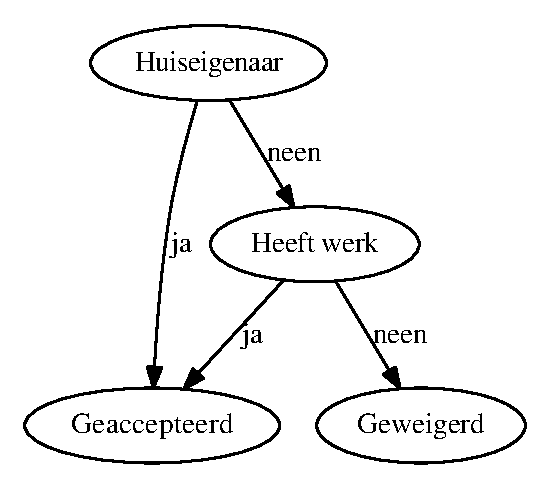
\includegraphics[width=0.6\textwidth]{res/ch5_dt_vb2.eps}
\caption{De beslissingsboom opgesteld door het algoritme}
\end{figure}

Tot nu toe zijn we ervan uitgegaan dat attributen discreet zijn. Het algoritme werkt echter ook met continue attributen. Dit kunnen we doen door met intervallen te werken. Het moeilijke hierbij is de keuze van de waarde die dient als onderverdeling van deze intervallen. Hiervoor gebruiken we opnieuw de informatiewinst. We sorteren eerst de waarden in onze dataset in toenemende volgorde: $\{v_1,v_2,...v_k\}$. Een van de mogelijke waarden voor de drempel is dan deze tussen $v_i$ en $v_{i+1}$. We proberen alle drempels en kiezen degene die de maximale winst oplevert. Het probleem bij deze aanpak is dat men zo kan blijven onderverdelen aangezien de waarden continu zijn.

Een laatste probleem bij het opstellen van beslissingsbomen is \emph{overfitting}. Hierbij is de boom teveel aangepast aan de trainingdata en niet genoeg aan het algemene geval. De symptomen hiervan zijn vaak duidelijk omdat de boom diep is en enorm veel takken bevat. Dit is vaak te wijten aan ruis of andere afwijkingen. Er zijn twee manieren om dit te vermijden:
\begin{enumerate}
\item Bij \emph{pre-pruning} wordt de constructie van de boom vroegtijdig gestart. De moeilijkheid hierbij is om te weten wanneer men moet stoppen.
\item Bij \emph{post-pruning} worden takken verwijderd van een reeds gemaakte boom gebaseerd op een statisch model dat de fouten per tak berekent.
\end{enumerate}

\section{K-nearest neighbour}
Een tweede algoritme voor \emph{supervised learning} dat we zullen bespreken is het \emph{K-nearest neighbour} algoritme. In tegenstelling tot bijvoorbeeld beslissingsbomen bouwt KNN geen model van de training data.

Algoritme \ref{algo:knn} beschrijft hoe dit gebruikt wordt in R en het resultaat van dit script is figuur \ref{figure:knn_after}.

\begin{algorithm}
\caption{Het kNN algoritme}
\label{algo:knn}
\begin{algorithmic}[1]
\Require D: Training data, d: het element dat geclassificeerd moet worden, k: Het aantal buren.
\Function{kNN}{D,d,k}
	\State bereken\_afstand($d,D$);
    \State $P$ = kies\_k\_dichtste($D$,k);
    \State d->klasse = meest\_frequente($P$);
\EndFunction
\end{algorithmic}
\end{algorithm}
Hierbij geven we $d$ dus een klasse door eerst alle afstanden in $D$ tot aan $d$ te berekenen. Hieruit kiezen we dan $k$ punten die we in de verzameling $P$ plaatsten. De klasse van $d$ stellen we dan gelijk aan de meest voorkomende klasse in $P$. We gaan er dus van uit dat de kans op klasse $c_j$, indien we $n$ kennen, gelijk is aan $\frac{n}{k}$.

\begin{equation}
p(c_j|d) = \frac{n}{k}
\end{equation}

Cruciaal hierbij is de keuze van de afstandsberekening. Het meest voor de hand liggende is natuurlijk de euclidische afstand, maar alternatieven---zoals de \emph{Manhattan distance}---zijn ook mogelijk. De keuze is vaak afhankelijk van de applicatie.

\emph{k} is meestal empirisch gekozen door handmatig te kiezen of via een controle set.

\begin{figure}[h]
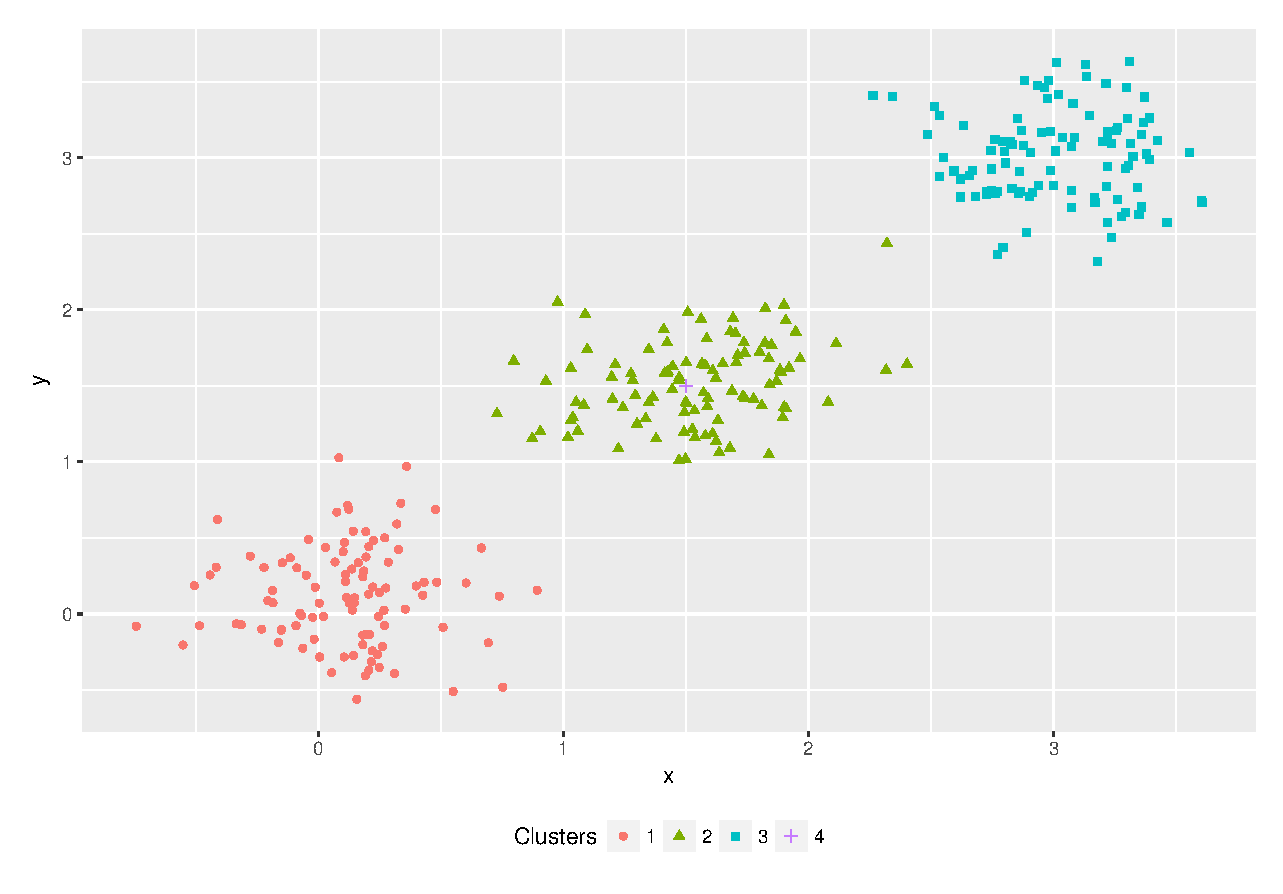
\includegraphics[width=\textwidth]{res/knn_before.eps}
\caption{De data voor het knn algoritme wordt toegepast.}
\label{figure:data-knn}
\end{figure}

\newpage
\paragraph{Voorbeeld} We maken gebruik van de \emph{package} FNN. Stel dat we reeds geclassificeerde data hebben, welke in figuur \ref{figure:data-knn} gevisualiseerd is. In de figuur zijn er 3 groepen met elk een klasse en 1 testpunt. De code om het punt te classificeren ziet er als volgt uit:

\inputminted{R}{code/knn.R}

\begin{figure}[h]
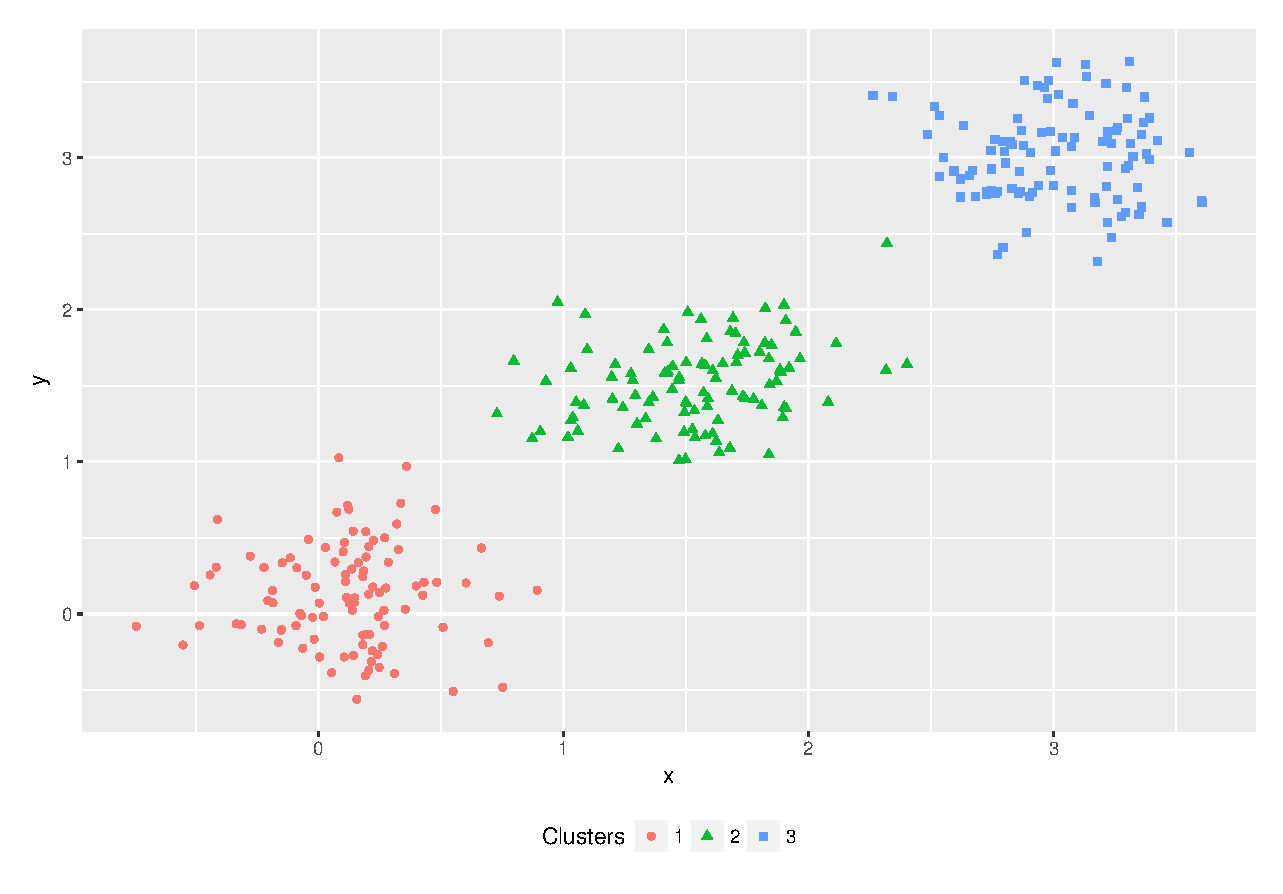
\includegraphics[width=\textwidth]{res/knn_after.eps}
\caption{De data nadat het KNN algoritme wordt toegepast: het punt behoord tot de juiste klasse.}
\label{figure:knn_after}
\end{figure}

\subsection{Bemerkingen bij KNN}
Het KNN algoritme heeft enkele voordelen:
\begin{itemize}
\item De eenvoudigheid. KNN is een zeer eenvoudig algoritme om te begrijpen en implementeren. Desondanks heeft KNN al heel wat goede resultaten opgeleverd.
\item KNN kan overweg met complexe grenzen tussen data.
\end{itemize}
Er zijn echter ook enkele nadelen aan verbonden.
\begin{itemize}
\item In tegenstelling tot bijvoorbeeld beslissingsbomen levert KNN geen begrijpbaar model op.
\item Omdat er geen model wordt gemaakt en de classificatie meteen gebeurt, is KNN traag tijdens deze classificatie.
\end{itemize}

\subsection{Besluit}
\emph{Supervised learning} is een reeks van technieken die reeds geclassificeerde data gebruikt om toekomstige classificaties te voorspellen. Twee van deze technieken hebben we besproken in deze cursus. Bij de eerste, beslissingsbomen, wordt er een boomstructuur opgesteld a.d.h.v. de trainingsdata waarna de testdata eenvoudig geclassificeerd kan worden. Bij de tweede techniek, KNN, krijgen we geen verstaanbaar model maar deze techniek werkt wel voor complexe data.
%
%Chapter 6: Information retrieval and web search
\chapter{Information retrieval and web search}
\emph{Information retrieval} of kortweg IR is een reeks van technieken die gebruikt worden om tekst te bewerken voordat deze gebruikt worden in data mining algoritmes. IR helpt gebruikers met behulp van \emph{queries} zodat deze informatie kunnen bijwinnen. Algemeen definieert men IR dus als de studie die de verzameling, verwerking, opslag en verspreiding van informatie mogelijk maakt.

Architecturaal kan men IR als volgt voorstellen:
\begin{figure}
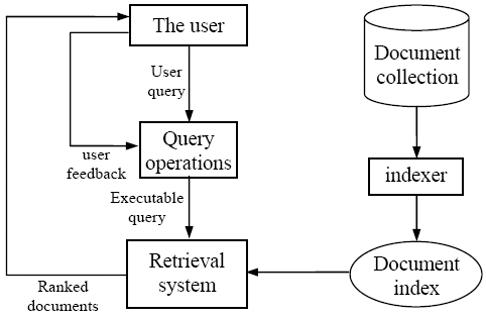
\includegraphics[width=0.8\textwidth]{res/IR}
\caption{De architectuur van IR.}
\end{figure}

Hierbij kan de gebruiker dus aan de hand van query's informatie opvragen. Gebaseerd op het document dat hij hierbij terugkrijgt kan de query dan eventueel aangepast worden. Er zijn verschillende soorten query's mogelijk:
\begin{itemize}
\item \textbf{Keyword queries}: Zoeken met kernwoorden zoals bijvoorbeeld op Google.
\item \textbf{Boolean queries}: AND, OR, NOT gebruiken om query's samen te stellen.
\item \textbf{Phrase queries}: Zoeken via zinnen.
\item \textbf{Proximity queries}: Zoeken naar woorden die normaal gezien vaak samen voorkomen.
\item \textbf{Full document queries}: Gebruikt bij bijvoorbeeld plagiaatcontrole.
\item \textbf{Natural language questions}: Gebruikt bij \emph{voice assistants} zoals Siri, Cortana, Alexa \dots
\end{itemize}

Een IR model bepaalt hoe een document en een query zijn opgebouwd. De meest voorkomende zijn booleaanse modellen, \emph{vector spac}e modellen en \emph{statistical language} modellen.
\section{Booleaans model}
Bij een booleaans model wordt elk document en elke query beschouwd als een groep van woorden. De volgorde waarin deze voorkomen is niet belangrijk.
Algemeen stellen we dat voor een groep documenten $D$ we $V = \{ t_1, t_2, ..., t_{|V|}\}$ defini\"eren als de woordenschat van deze documenten. 
Aan elk woord $t_i$ uit document $d_j \in D$ wordt een gewicht $w_{ij} = 1$ toegekend. Voor termen die niet voorkomen in document $d_j$ is het gewicht gelijk aan nul. Het document is dus gelijk aan: 

\begin{equation}
d_j = \left( w_{1j},w_{2j},..,w_{|V|j} \right)
\end{equation}

Met behulp van booleaanse operatoren kunnen query's op opgebouwd worden; waarbij het gewicht $w_{ij}$ in beschouwing wordt genomen. Ieder document waarvoor het resultaat \emph{true} is, wordt opgehaald en teruggegeven. De resultaten voor deze query's zijn vaak slecht omdat er geen rekening wordt gehouden met de frequentie van woorden. De gewichten zijn immers 0 of 1. Een voorbeeld van zo een query: (\emph{voetbal} AND (NOT \emph{anderlecht})).

\section{Vector space model}
Bij een \emph{vector space model} of VSM wordt een document opnieuw voorgesteld als een groep van woorden. Elk document is een vector met daarin per woord een gewicht. In tegenstelling tot bij het booleaans model is het gewicht niet gewoon 0 of 1. Om dit gewicht te berekenen maken we gebruik van een \emph{Term Frequency} (TF) model. De definitie  hiervan is eenvoudig; het gewicht van een term $t_i$ in een document $d_j$ is het aantal keren dat $t_i$ voorkomt in $d_j$ voorgesteld in $f_{ij}$. We kunnen deze waarden ook normaliseren. We spreken dan van TF-IDF model. IDF staat voor \emph{Inverse Document Frequency}. De gewichten bij TF-IDF worden dan als volgt berekend:
\begin{equation}
tf_{ij} = \frac{f_{ij}}{max_{f_j \in d_j}f_j}
\end{equation}
Met $N$ het aantal documenten en $df_i$ het aantal documenten dat $t_i$ bevat:
\begin{equation}
idf_i = \log{ \frac{N}{df_i}}
\end{equation}
Wordt het gewicht:
\begin{equation}
w_{ij} = tf_{ij} \cdot idf_i
\end{equation}
We houden dus niet alleen rekening met de frequentie van een woord in 1 document, maar kijken over alle documenten heen.

Het opstellen van een query is bij VSM is minder eenvoudig dan bij een booleaans model en maakt gebruik van een inwendig product (dot product) tussen 2 vectoren. We stellen immers zowel de query  als het document voor als een vector. Hoe beter de vectoren overeenkomen, hoe groter de cosinus tussen deze vectoren. Algemeen berekenen we de overeenkomst als

\begin{equation}
\cos{\left(d_j,q\right)} = \frac{d_j \cdot q}{||d_j|| ||q||} =
\frac{\sum_{i=1}^{|V|}{w_{ij} w_{iq}}}{\sqrt[]{
\sum_{i=1}^{|V|}{ w_{ij}^2}
\sum_{i=1}^{|V|}{w_{iq}^2}
}}
\end{equation}

%
\paragraph{Voorbeeld}

Stel dat we volgende woordenschat hebben: \emph{hardware,software,users} en volgende set van documenten met als query: 'hardware and software':

\begin{table}[h]
\centering
\caption{Een verzameling met applicaties $D$.}
\label{tabel:sl_ex1}
\begin{tabular}{c|c}
\textbf{Set} & \textbf{Inhoud} \\
$A_1$ & $\{1,0,0\}$ \\
$A_2$ & $\{0,1,0\}$ \\
$A_3$ & $\{0,0,1\}$ \\
$A_4$ & $\{1,1,0\}$ \\
$A_5$ & $\{1,0,1\}$ \\
$A_6$ & $\{0,1,1\}$ \\
$A_7$ & $\{1,1,1\}$ \\
$A_8$ & $\{1,0,1\}$ \\
$A_9$ & $\{0,1,1\}$
\end{tabular}
\end{table}
%

Bij het booleaanse model krijgen we dan $A_4$ en $A_7$ terug. We kijken immers gewoon of de term voorkomt en gebruiken een AND-relatie. 

Bij VSM berekenen we telkens de cosinus tussen de twee vectoren. De query---voorgesteld als vector---ziet er als volgt uit: 
\begin{equation}
q(1,1,0)
\end{equation}

We krijgen de volgende waarden per document:

\begin{table}[h]
\centering
\caption{Een verzameling met applicaties $D$.}
\label{tabel:sl_ex1}
\begin{tabular}{c|c|c}
\textbf{Set} & \textbf{Inhoud} & \textbf{cos} \\
$A_1$ & $\{1,0,0\}$ & 0,71 \\
$A_2$ & $\{0,1,0\}$ & 0,71\\
$A_3$ & $\{0,0,1\}$ & 0\\
$A_4$ & $\{1,1,0\}$ & 1\\
$A_5$ & $\{1,0,1\}$ & 0,5\\
$A_6$ & $\{0,1,1\}$ & 0,5\\
$A_7$ & $\{1,1,1\}$ & 0,82\\
$A_8$ & $\{1,0,1\}$ & 0,5\\
$A_9$ & $\{0,1,1\}$ & 0,5\\
\end{tabular}
\end{table}

Hieruit krijgen we dan de volgende documenten terug: $A_1,A_2,A_4,A_5,A_6,A_7,A_8,A_9$.

\section{Text processing}
Indien we het huidig model zouden gebruiken, dan zou dit geen goede resultaten geven. Documenten bevatten vaak woorden die geen waarde toevoegen: stopwoorden. Het verwijderen van deze stopwoorden verhoogt de effici\"entie en accuraatheid van het zoeksysteem. Men kan lijsten met stopwoorden online vinden. Voor sommige toepassingen wordt bovenop deze lijst nog een extra reeks woorden toegevoegd die men ook als stopwoorden beschouwd. 

Naast stopwoorden moet men ook nog \emph{stemming} toepassen, waarmee herleid wordt naar de stam van een woord. Woorden zoals loop, loper, loopt, gelopen \dots zijn kleine veranderingen op het woord loop. \emph{Stemming} maakt het mogelijk om dit allemaal terug te laten wijzen op hetzelfde basiswoord. Ook hier is het doel om de effici\"entie te verhogen en de grootte van de index te verkleinen. Per taal is er een reeks technieken beschikbaar om aan \emph{stemming} te doen. Zo kan men in het Engels bij woorden die op -ing eindigen, dit laatste wegdoen.

Tot slot kan men opnieuw TF-IDF toepassen om de termen bij te houden in de index.

Zoals gezien zijn er meerdere methoden om op queries te reageren. We hebben dus een manier nodig om deze te evalueren. Hierbij stellen we ons 2 vragen:
\begin{itemize}
\item Is elke opgehaald document relevant?
\item Zijn alle relevante documenten opgehaald?
\end{itemize}
De eerste vraag heeft betrekking tot de nauwkeurigheid van de zoekopdracht, terwijl de tweede betrekking heeft op de volledigheid. Dit wordt duidelijk gemaakt in de volgende figuur:

\begin{figure}[h]
\centering
\caption{Nauwkeurigheid en volledigheid van een zoekopdracht.}
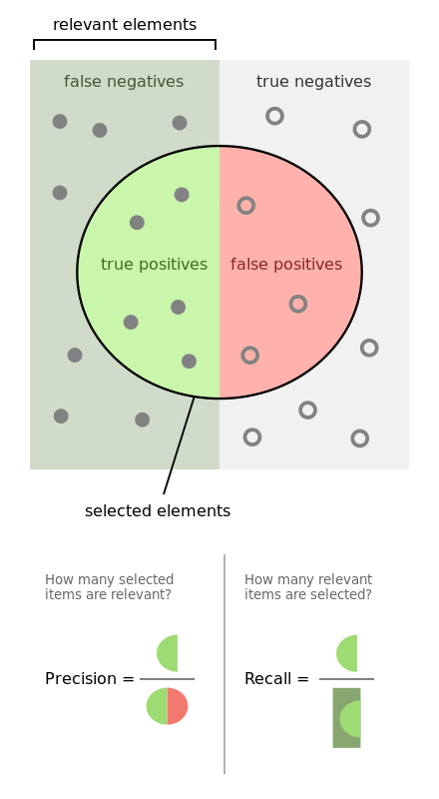
\includegraphics[width=0.55\textwidth]{res/evaluation_queries}
\end{figure}

\newpage
We kunnen deze algoritmes met elkaar vergelijken met de volgende formule; waarmee we dan grafieken kunnen opstellen om de verschillende algoritmes visueel met elkaar te vergelijken.

\begin{equation}
\overline{p}\left(r_i\right)=\frac{1}{|Q|}\sum_{j=1}^{|Q|}{p_j(r_i)}
\end{equation}

%
\subsection{Inverted index}
Men kan een zoekopdracht via het internet beschouwen als een groot IR systeem. Hierbij moet een \emph{webcrawler} alle webpagina's die deze tegenkomt opslaan in wat men een ge\"inverteerde indexing database noemt.
Voor ieder item kan een lijst met documenten worden bijgehouden waar het item in voorkomt. Dit is een ge\"inverteerde index, wat als voordeel heeft dat het vinden van documenten in vaste tijdsduur kan gebeuren. Daarnaast kunnen meerdere query-elementen ook eenvoudig verwerkt worden.

Als we een query $q$ beschouwen, dan omvat zoeken de volgende stappen:

\begin{enumerate}
\item \textbf{Vocabulary search}: Zoek alle woorden in $q$ in de ge\"inverteerde index.
\item \textbf{Resultaten mergen}: \emph{Merge} de resulaten die alle of enkele woorden uit $q$ bevatten.
\item \textbf{Rank score computation}: Order de documenten.
\end{enumerate}


%

%%
% The back matter contains appendices, bibliographies, indices, glossaries, etc.

%\backmatter

%	 \bibliography{sample-handout}
% \bibliographystyle{plainnat}


\end{document}

